% Options for packages loaded elsewhere
\PassOptionsToPackage{unicode}{hyperref}
\PassOptionsToPackage{hyphens}{url}
%
\documentclass[
  a4paper,
]{scrbook}

\usepackage{amsmath,amssymb}
\usepackage{iftex}
\ifPDFTeX
  \usepackage[T1]{fontenc}
  \usepackage[utf8]{inputenc}
  \usepackage{textcomp} % provide euro and other symbols
\else % if luatex or xetex
  \usepackage{unicode-math}
  \defaultfontfeatures{Scale=MatchLowercase}
  \defaultfontfeatures[\rmfamily]{Ligatures=TeX,Scale=1}
\fi
\usepackage{lmodern}
\ifPDFTeX\else  
    % xetex/luatex font selection
  \setmainfont[]{Latin Modern Roman}
  \setsansfont[]{Latin Modern Roman}
\fi
% Use upquote if available, for straight quotes in verbatim environments
\IfFileExists{upquote.sty}{\usepackage{upquote}}{}
\IfFileExists{microtype.sty}{% use microtype if available
  \usepackage[]{microtype}
  \UseMicrotypeSet[protrusion]{basicmath} % disable protrusion for tt fonts
}{}
\makeatletter
\@ifundefined{KOMAClassName}{% if non-KOMA class
  \IfFileExists{parskip.sty}{%
    \usepackage{parskip}
  }{% else
    \setlength{\parindent}{0pt}
    \setlength{\parskip}{6pt plus 2pt minus 1pt}}
}{% if KOMA class
  \KOMAoptions{parskip=half}}
\makeatother
\usepackage{xcolor}
\setlength{\emergencystretch}{3em} % prevent overfull lines
\setcounter{secnumdepth}{5}
% Make \paragraph and \subparagraph free-standing
\ifx\paragraph\undefined\else
  \let\oldparagraph\paragraph
  \renewcommand{\paragraph}[1]{\oldparagraph{#1}\mbox{}}
\fi
\ifx\subparagraph\undefined\else
  \let\oldsubparagraph\subparagraph
  \renewcommand{\subparagraph}[1]{\oldsubparagraph{#1}\mbox{}}
\fi


\providecommand{\tightlist}{%
  \setlength{\itemsep}{0pt}\setlength{\parskip}{0pt}}\usepackage{longtable,booktabs,array}
\usepackage{calc} % for calculating minipage widths
% Correct order of tables after \paragraph or \subparagraph
\usepackage{etoolbox}
\makeatletter
\patchcmd\longtable{\par}{\if@noskipsec\mbox{}\fi\par}{}{}
\makeatother
% Allow footnotes in longtable head/foot
\IfFileExists{footnotehyper.sty}{\usepackage{footnotehyper}}{\usepackage{footnote}}
\makesavenoteenv{longtable}
\usepackage{graphicx}
\makeatletter
\def\maxwidth{\ifdim\Gin@nat@width>\linewidth\linewidth\else\Gin@nat@width\fi}
\def\maxheight{\ifdim\Gin@nat@height>\textheight\textheight\else\Gin@nat@height\fi}
\makeatother
% Scale images if necessary, so that they will not overflow the page
% margins by default, and it is still possible to overwrite the defaults
% using explicit options in \includegraphics[width, height, ...]{}
\setkeys{Gin}{width=\maxwidth,height=\maxheight,keepaspectratio}
% Set default figure placement to htbp
\makeatletter
\def\fps@figure{htbp}
\makeatother

\usepackage{booktabs}
\usepackage{longtable}
\usepackage{array}
\usepackage{multirow}
\usepackage{wrapfig}
\usepackage{float}
\usepackage{colortbl}
\usepackage{pdflscape}
\usepackage{tabu}
\usepackage{threeparttable}
\usepackage{threeparttablex}
\usepackage[normalem]{ulem}
\usepackage{makecell}
\usepackage{xcolor}
\usepackage{fancyhdr}
\usepackage{titling}
\usepackage{pdflscape}
\usepackage{geometry}
\setlength{\droptitle}{-2cm}
\preauthor{
  \begin{center}
  \Large
  \vspace{10mm}
  by
  \vspace{20mm}
}
\postauthor{
  \end{center}
  \vfill
}

\predate{
  \begin{center}
  A thesis 
  submitted in partial fulfilment of the \\
  requirements of the degree of \\
  Doctor of Philosophy in Physics\\               % Degree
  School of Physical and Chemical Sciences\\          % Department
  Te Herenga Waka - Victoria University of Wellington\\                       % University 
  \vspace{5mm}
}
\postdate{
  \\
  \includegraphics[width=3in,height=1.5in]{figures/VUW-logo.png}\\
  \end{center}
  }

\renewcommand{\topfraction}{.8}
\renewcommand{\bottomfraction}{.7}
\renewcommand{\textfraction}{.15}
\renewcommand{\floatpagefraction}{.8}
\setcounter{topnumber}{3}
\setcounter{bottomnumber}{3}
\setcounter{totalnumber}{4}

\clubpenalty=9996
\widowpenalty=9999
\makeatletter
\makeatother
\makeatletter
\@ifpackageloaded{bookmark}{}{\usepackage{bookmark}}
\makeatother
\makeatletter
\@ifpackageloaded{caption}{}{\usepackage{caption}}
\AtBeginDocument{%
\ifdefined\contentsname
  \renewcommand*\contentsname{Table of contents}
\else
  \newcommand\contentsname{Table of contents}
\fi
\ifdefined\listfigurename
  \renewcommand*\listfigurename{List of Figures}
\else
  \newcommand\listfigurename{List of Figures}
\fi
\ifdefined\listtablename
  \renewcommand*\listtablename{List of Tables}
\else
  \newcommand\listtablename{List of Tables}
\fi
\ifdefined\figurename
  \renewcommand*\figurename{Figure}
\else
  \newcommand\figurename{Figure}
\fi
\ifdefined\tablename
  \renewcommand*\tablename{Table}
\else
  \newcommand\tablename{Table}
\fi
}
\@ifpackageloaded{float}{}{\usepackage{float}}
\floatstyle{ruled}
\@ifundefined{c@chapter}{\newfloat{codelisting}{h}{lop}}{\newfloat{codelisting}{h}{lop}[chapter]}
\floatname{codelisting}{Listing}
\newcommand*\listoflistings{\listof{codelisting}{List of Listings}}
\makeatother
\makeatletter
\@ifpackageloaded{caption}{}{\usepackage{caption}}
\@ifpackageloaded{subcaption}{}{\usepackage{subcaption}}
\makeatother
\makeatletter
\@ifpackageloaded{tcolorbox}{}{\usepackage[skins,breakable]{tcolorbox}}
\makeatother
\makeatletter
\@ifundefined{shadecolor}{\definecolor{shadecolor}{rgb}{.97, .97, .97}}
\makeatother
\makeatletter
\makeatother
\makeatletter
\makeatother
\ifLuaTeX
  \usepackage{selnolig}  % disable illegal ligatures
\fi
\usepackage[citestyle = ieee,urldate = iso8601]{biblatex}
\addbibresource{references.bib}
\IfFileExists{bookmark.sty}{\usepackage{bookmark}}{\usepackage{hyperref}}
\IfFileExists{xurl.sty}{\usepackage{xurl}}{} % add URL line breaks if available
\urlstyle{same} % disable monospaced font for URLs
\hypersetup{
  pdftitle={Developing an Insect Odorant Receptor Bioelectronic Nose for Vapour-Phase Detection},
  pdfauthor={Eddyn Oswald Perkins Treacher},
  hidelinks,
  pdfcreator={LaTeX via pandoc}}

\title{Developing an Insect Odorant Receptor Bioelectronic Nose for
Vapour-Phase Detection}
\author{Eddyn Oswald Perkins Treacher}
\date{Dec 2024}

\begin{document}
\frontmatter

\maketitle

\clearpage
\newpage
\thispagestyle{empty} % Hide header and footer on this page
\mbox{~}
\clearpage
\newpage

%----------------------------------------------
%   Abstract
%----------------------------------------------

\thispagestyle{plain}

\begin{flushleft}
% Manually add a section to the table of contents
\pagenumbering{roman}
\addcontentsline{toc}{chapter}{Abstract}
\huge\textbf{Abstract}
\end{flushleft}

\vspace*{\baselineskip}

The ability to detect volatile organic compounds in a highly sensitive and selective manner is desirable for applications as varied as diagnosis of illnesses at a remote clinic, monitoring of air in an industrial setting, or identification of invasive organisms at a biosecurity checkpoint. Historically, animal noses have been used for such tasks, as their combined sensitivity and selectivity are superior to traditional artificial sensors. However, training and deploying animals in such situations is both time and cost intensive. In recent years, an improved understanding of \textit{in vivo} biological sensing has driven efforts to mimic these highly efficient processes in an artificial sensor format. \\[5pt] To this end, a “bioelectronic nose” was developed. This sensor uses an artificial transducer to amplify responses of an insect odorant receptor protein to specific volatile compounds. Thin-film transistors were used as the amplifier element, given their low cost, small size and extreme sensitivity. Various thin-film morphologies were compared, and their suitability for bioelectronic nose development assessed. Transducers made using a novel steam-assisted thin-film deposition technique were found to have highly consistent device-to-device electrical properties relative to other films. Films made using this process typically showed more surface contamination than other morphologies, but their high sensitivity was nonetheless confirmed with a non-specific sensing series in an aqueous environment. \\[5pt] One of the major challenges encountered in this thesis was variability in the quality of sensor functionalisation. Raman spectroscopy and fluorescence microscopy confirmed an existing non-covalent attachment method could successfully immobilise nanodiscs onto the transistor channel region. However, various sensors functionalised using the same procedure often exhibited no sensing activity. Extensive electrical characterisation indicated the presence of an unidentified contamination layer preventing electrical interaction between the insect odorant receptors and transducer thin-film. It was shown that this layer was unlikely to be directly associated with the thin-film morphology used for the transducer. \\[5pt] Subsequently, an alternative biotin-based non-covalent method was used for functionalisation of the proteins, which eliminated several possible contamination sources. This alternative biotin-based method was used to demonstrate successful aqueous sensing of femtomolar concentrations of methyl salicylate by an iOR10a-functionalised device. When tested in a custom-built vapour delivery system, a similar bioelectronic sensor was shown to be highly sensitive to the target vapour. However, consistent reproduction of the biotin-based method was challenging due to the harsh cleaning method involved. It was therefore difficult to determine conclusively whether sensor responses were selective. By finding new, systematic approaches to address the major barriers to sensor success carefully identified in this work, there are promising signs that a highly reliable vapour-phase bioelectronic nose can be produced.

%\fancyhf{} %clear all headers and footers fields
%\thispagestyle{fancy} % Change header and footer on this page
%\renewcommand{\headrulewidth}{0pt}
%\fancyhead[L]{\textit{Abstract}} % Set header content
%\fancyfoot[L]{\thepage} %prints the page number on the right side of the header

\clearpage
\newpage
\thispagestyle{empty} % Hide header and footer on this page
\mbox{~}
\clearpage
\newpage


%----------------------------------------------
%   Acknowledgement
%----------------------------------------------

\thispagestyle{plain}

\begin{flushleft}
% Manually add a section to the table of contents
\addcontentsline{toc}{chapter}{Acknowledgements}
\huge\textbf{Acknowledgements}
\end{flushleft}

\vspace*{\baselineskip}

I would first like to acknowledge the lands of my ancestors, and the lands of the sovereign first peoples to which my ancestors travelled. We each come from the land, live off the land and return to the land.\\[5pt]
\textit{Noon of Essex to Warrang, on the Friends, Autumn 1811} \\[5pt]
\textit{Cave of Cambridgeshire to Warrang, on the Royal Charlotte, Autumn 1825} \\[5pt]
\textit{Boyce of Suffolk to Warrang, 1832} \\[5pt] 
\textit{Charlton of Northumberland to Warrang, on the Clyde, Spring 1834} \\[5pt]
\textit{Prouse of Devonshire to Pito-one, on the Duke of Roxburgh, Summer 1840} \\[5pt]
\textit{Ebden of Devonshire to Pito-one, on the Tyne, Winter 1841} \\[5pt]
\textit{Collis of Hampshire to Pito-one, on the Birman, Autumn 1842} \\[5pt]
\textit{Swann of Loch Garman to Te Whanganui-a-Tara, 1844} \\[5pt] 
\textit{Blythe of Berkshire to Whakatū, circa 1846} \\[5pt]
\textit{Innes of Berkshire to Naarm, on the Sacramento, Autumn 1853} \\[5pt]
\textit{Sheppard of Gloucestershire to Naarm, 1853} \\[5pt] 
\textit{Bruce of London to Naarm, on the Omega, Autumn 1855} \\[5pt]
\textit{Quennell of Surrey to Warrang, on the Asiatic, Winter 1855} \\[5pt]
\textit{Barr of Glasgow to Kōpūtai, on the Sir Edward Paget, Winter 1856} \\[5pt] 
\textit{Perkins of London to Te Whanganui-a-Tara, on the Matoaka, Spring 1859} \\[5pt]
\textit{McKee of Antrim to Tāmaki Makaurau, on the Indian Empire, Spring 1862} \\[5pt]
\textit{Sandilands of Peeblesshire to Ōtepoti, circa 1864} \\[5pt] 
\textit{Treacher of Berkshire to Te Whanganui-a-Tara, on the Wild Duck, Summer 1865} \\[5pt]
\textit{McTaggart of Argyllshire to Kōpūtai, on the Edward P. Bouverie, Autumn 1869} \\[5pt] 
\textit{Chapman of Kent to Whakatū, on the Adamant, Winter 1874} \\[5pt]
\textit{Cheel of London to Whakatū, on the Queen Bee, Winter 1877} \\[5pt]  
\textit{Hutchison of Aberdeen to Tarntanya, before 1882.} \\[5pt] 
I chose to start my doctoral studies just a few months into a global pandemic. Completing a challenging project with a worldwide crisis in the background might have been impossible without the supervision of AProf. Natalie Plank. Her ability to adapt to and overcome any problem has taught me that there is no situation which is truly unmanageable. I am deeply grateful for her leadership throughout a time of particular chaos. \newpage
\fancyhf{} %clear all headers and footers fields
\thispagestyle{fancy} % Change header and footer on this page
\renewcommand{\headrulewidth}{0pt}
\fancyhead[L]{\textit{Acknowledgements}} % Set header content
\fancyfoot[L]{\thepage} %prints the page number on the left side of the header 
I started this project with minimal formal training in biological science, coming from a primarily physics and engineering background. \\[5pt] The immense support I received from Melissa Jordan and Colm Carraher from the Institute for Plant and Food Research (PFR) to complete this project meant that this was not an issue, and I thank them both immensely for this. \\[5pt] I would not have been able to begin this thesis without the financial backing and support I received from PFR and the Better Border Biosecurity (B3) programme. In particular, I am very grateful to Andrew Kralicek, formerly with PFR and now at Scentian Bio, and the ex-Director of B3, David Teulon, for helping to secure funding for my project. I would also like to thank the donor of the Ernest Marsden Scholarship in Physics for their significant financial support. \\[5pt] There are many incredibly supportive people who I worked alongside during my project. I would like to start off by thanking Rifat Ullah, whose mentoring and kindness encouraged me to pursue further study. His work on the initial design and setup of the vapour delivery system was invaluable to me throughout this project. I am also especially grateful to Alex Puglisi, for constructing the mechanical elements of the vapour delivery system and giving me extensive feedback on the system design. I would like to thank Peter Coard, for his advice and guidance when constructing the electrical elements of the vapour delivery system. I thank Selvan Murugathas, too, for his advice on constructing the insect odorant receptor sensors, as well as Damon Colbert and Valentina Lucarelli, who provided the insect odorant receptor nanodiscs used in this work. \\[5pt] Thank you to AProf. Ben Ruck, my supportive secondary supervisor, and to AProf. Franck Natali, for always asking about my thesis in the tearoom. Thank you to Gideon Gouws for his friendly encouragement and advice. For their substantial technical assistance and mentoring during this project, I thank Alan Rennie, Grant Franklin, Chris Lepper, Rashika Gunasekara, Pete Jebson and Sushila Pillai from VUW, Andrew Chan from PFR, AProf. Charles Unsworth from the University of Auckland, and Prof. Simon Brown and his nanomaterials group from the University of Canterbury. \\[5pt] I was lucky enough to start my doctoral program just as a group of supportive and talented senior students were finishing, and finished just as a group of enthusiastic and talented new doctoral students were starting. A special thanks to Jenna Nyugen, Erica Happe and Erica Cassie for teaching me the fabrication processes and characterisation procedures that made this thesis happen; and a special thanks to Marissa Dierkes, Danica Fontein, Sangar Begzaad and Alireza Zare, for their incredible support throughout the thesis writing process. I am also thankful for the assistance of the cleanroom group interns over the course of my PhD, including Liam, Hayden and Lotte. I would further like to thank everyone else I shared an office with and worked alongside, including Jackson, Will, Roshni, Ali, Sam, Kira, Catherine, Martin, Janani, Ted, Kiri and Joe. \\[5pt] A massive thank you to Openstar Technologies. It has been an honour to work on a cutting-edge plasma physics project right here in Te Whanganui-a-Tara. A particularly big thank you to Ratu, Darren and Thomas for having me as part of the plasma physics team. Thank you also to the other Openstar interns, in particular the other plasma physics interns, Valentina, Benjy and Chris. I wish you success in all your dipole-confined plasma related endeavours. \\[5pt] I want to thank Shodokan Aikido New Zealand for their support throughout this thesis, in particular for the once-in-a-lifetime opportunity to travel to Osaka to be graded for first-dan by Nariyama Shihan. Thanks for all the training and support, Ian. Thank you to all the friends and family, old and new, who have supported me over these wild past few years. You know who you are. \\[5pt] Thank you to my brother, Keeson, and to my parents, Hilary and Phillip. Your support means everything to me, and I would not be where I am today without you. Our Friday lunchtime cafe visits inspired and motivated me throughout the doctoral program. Thank you, thank you, thank you for your love, your compassion, and for being there for me. \\[5pt] Finally, thank you Nina. Your love has kept me going through the most difficult and most wonderful times over the last three and a half years. You are the light of my life, and I am so happy to have taken on this challenge with you by my side. \\[5pt] Arohanui and peace to you all, Eddyn (Ned)

\fancyhf{} %clear all headers and footers fields
\thispagestyle{fancy} % Change header and footer on this page
\renewcommand{\headrulewidth}{0pt}
\fancyhead[R]{\textit{Acknowledgements}} % Set header content
\fancyfoot[R]{\thepage} %prints the page number on the right side of the header

\clearpage
\newpage
\thispagestyle{empty} % Hide header and footer on this page
\mbox{~}
\clearpage
\newpage

\pagestyle{headings}

\ifdefined\Shaded\renewenvironment{Shaded}{\begin{tcolorbox}[boxrule=0pt, frame hidden, breakable, interior hidden, borderline west={3pt}{0pt}{shadecolor}, enhanced, sharp corners]}{\end{tcolorbox}}\fi

\renewcommand*\contentsname{Table of Contents}
{
\setcounter{tocdepth}{2}
\addcontentsline{toc}{chapter}{Table of Contents}
\tableofcontents
}
\listoffigures
\addcontentsline{toc}{chapter}{List of Figures}
\listoftables
\addcontentsline{toc}{chapter}{List of Tables}

\clearpage
\newpage
\thispagestyle{empty} % Hide header and footer on this page
\mbox{~}
\clearpage
\newpage

%----------------------------------------------
%   List of Abbreviations
%----------------------------------------------

\thispagestyle{plain}

\begin{flushleft}
% Manually add a section to the table of contents
\addcontentsline{toc}{chapter}{List of Abbreviations}
\huge\textbf{List of Abbreviations}
\end{flushleft}

\vspace*{\baselineskip}

\begin{table}[H]
  \begin{tabular}{@{}p{0.25\textwidth} p{0.75\textwidth}@{}}  % Adjust the width as needed
    2D  & 2-Dimensional  \\[5pt]
    Ab  & Antibody  \\[5pt]
    AB  & Amyl Butyrate  \\[5pt]
    AB-NTA  & N$\alpha$,N$\alpha$-Bis(carboxymethyl)-\textit{L}-lysine hydrate  \\[5pt]
    AFM  & Atomic Force Microscope/Microscopy  \\[5pt]
    AH  & Absolute Humidity  \\[5pt]
    Avi-tag  & Avidin-tag  \\[5pt]
    BMIM  & 1-butyl-3-methylimidazolium bis(trifluoromethylsulfonyl)imide  \\[5pt]
    BWF  & Breit-Wigner-Fano  \\[5pt]
    CAD  & Computer Aided Design \\[5pt]
    CNT  & Carbon Nanotube  \\[5pt]
    CVD  & Chemical Vapour Deposition  \\[5pt]
    Cy3  & Cyanine 3  \\[5pt]
    DAN  & 1,5-diaminonaphthalene  \\[5pt]
    DAQ  & Data Acquisition Input/Output Module  \\[5pt]
    DCB  & 1,2-dichlorobenzene  \\[5pt]
    DI  & Deionised  \\[5pt]
    DMF  & Dimethylformamide   \\[5pt]
    DMSO  & Dimethylsulfoxide   \\[5pt]
    DMT-MM   & 4-(4,6-dimethoxy-1,3,5-triazin-2-yl)-4 methylmorpholinium chloride \\[5pt]
    DMMP  & Dimethyl Methylphosphonate  \\[5pt]
    DNA  & Deoxyribonucleic Acid  \\[5pt]
    E2Hex  & \textit{trans}-2-hexan-1-al  \\[5pt]
    EB  & Ethyl Butyrate  \\[5pt]
    EDC  & 1-Ethyl-3-(3-dimethylaminopropyl)carbodiimide  \\[5pt]
    EDL  & Electric Double Layer  \\[5pt]
    EIS  & Electrochemical Impedance Spectroscopy  \\[5pt]
    EtHex  & Ethyl Hexanoate  \\[5pt]
  \end{tabular}
\end{table}

\newpage
\fancyhf{} %clear all headers and footers fields
\thispagestyle{fancy} % Change header and footer on this page
\renewcommand{\headrulewidth}{0pt}
\fancyhead[L]{\textit{List of Abbreviations}} % Set header content
\fancyfoot[L]{\thepage} %prints the page number on the right side of the header
\begin{table}[H]
  \begin{tabular}{@{}p{0.25\textwidth} p{0.75\textwidth}@{}}  % Adjust the width as needed
    EtOH  & Ethanol  \\[5pt]
    FET  & Field-Effect Transistor  \\[5pt]
    FITC  & Fluorescein isothiocyanate  \\[5pt]
    GA  & Glutaraldehyde  \\[5pt]
    GFET  & Graphene Field-Effect Transistor  \\[5pt]
    GFP  & Green Fluorescent Protein  \\[5pt]
    GPCR  & G-protein Coupled Receptor  \\[5pt]
    HEK  & Human Embryonic Kidney  \\[5pt]
    His-tag  & Histidine-tag  \\[5pt]
    hOR  & Human Odorant Receptor  \\[5pt]
    HPLC  & High-performance Liquid Chromatography   \\[5pt]
    iOR  & Insect Odorant Receptor  \\[5pt]
    IPA  & Isopropanol  \\[5pt]
    LOD  & Limit of Detection  \\[5pt]
    m-CNT  & Metallic Carbon Nanotube   \\[5pt]
    MeOH  & Methanol   \\[5pt]
    MeSal  & Methyl Salicylate   \\[5pt]
    MFC  & Mass Flow Controller   \\[5pt]
    mOR  & Mouse Odorant Receptor  \\[5pt]
    MOSFET  & Metal-Oxide-Semiconductor Field-Effect Transistor  \\[5pt]
    MSP  & Membrane Scaffold Protein  \\[5pt]
    MWCNT  & Multi-Walled Carbon Nanotube  \\[5pt]
    ND  & Nanodisc  \\[5pt]
    NHS  & N-Hydroxysuccinimide  \\[5pt]
    NHSS  & N-hydroxysulfosuccinimide   \\[5pt]
    NMR  & Nuclear Magnetic Resonance  \\[5pt]
    NSB  & Non-Specific Binding   \\[5pt]
    NTA  & Nitrilotriacetic Acid   \\[5pt]
    OBP  & Odorant Binding Protein  \\[5pt]
    OR  & Odorant Receptor  \\[5pt]
    ORCO  & Odorant Receptor Co-Receptor  \\[5pt]
  \end{tabular}
\end{table}

\newpage
\fancyhf{} %clear all headers and footers fields
\thispagestyle{fancy} % Change header and footer on this page
\renewcommand{\headrulewidth}{0pt}
\fancyhead[R]{\textit{List of Abbreviations}} % Set header content
\fancyfoot[R]{\thepage} %prints the page number on the right side of the header
\begin{table}[H]
  \begin{tabular}{@{}p{0.25\textwidth} p{0.75\textwidth}@{}}  % Adjust the width as needed
    PBA  & 1-Pyrenebutyric Acid  \\[5pt]
    PBASE  & 1-Pyrenebutanoic Acid N-hydroxysuccinimide Ester  \\[5pt]
    PBS  & Phosphate-Buffered Saline  \\[5pt]
    PCB  & Printed Circuit Board   \\[5pt]
    PDL & Poly-\textit{D}-lysine  \\[5pt]
    PDMS  & Polydimethylsiloxane   \\  [5pt]
    PEG  & Polyethylene Glycol  \\[5pt] 
    PID  & Photoionisation Detector  \\[5pt] 
    PLL  & Poly-\textit{L}-lysine  \\[5pt]
    PPB  & Pyrene-PEG-Biotin  \\[5pt]
    PPF  & Pyrene-PEG-FITC  \\[5pt]
    PPN  & Pyrene-PEG-NTA  \\[5pt]
    PPR  & Pyrene-PEG-Rhodamine  \\[5pt]
    PTFE  & Polytetrafluoroethylene (Teflon™)  \\[5pt]
    PVC  & Polyvinyl chloride  \\[5pt]
    QCM  & Quartz Crystal Microbalance  \\[5pt]
    RH  & Relative Humidity  \\[5pt]
    RHI  & Relative Humidity and Temperature Indicator  \\[5pt] 
    RNA  & Ribonucleic Acid   \\[5pt]
    SAW  & Surface Acoustic Wave   \\[5pt]
    s-CNT  & Semiconducting Carbon Nanotube   \\[5pt]
    SEM  & Scanning Electron Microscope/Microscopy   \\[5pt]
    SMU  & Source Measure Unit   \\[5pt]
    SPR  & Surface Plasmon Resonance   \\[5pt]
    SWCNT  & Single-Walled Carbon Nanotube   \\[5pt]
    TFTFET  & Thin-Film Field-Effect Transistor  \\[5pt]
    TMAH  & Tetramethylammonium hydroxide  \\[5pt]
    TX  & Transfer Characteristics  \\[5pt]
    UV  & Ultraviolet  \\[5pt]
    VI  & Virtual Instrument  \\[5pt]
    VUAA1  & N-(4-Ethylphenyl)-2-{[4-ethyl-5-(pyridin-3-yl)-4H-1,2,4-triazol-3-yl]sulfanyl}acetamide  \\[5pt] 
  \end{tabular}
\end{table}

\clearpage
\newpage
\thispagestyle{empty} % Hide header and footer on this page
\mbox{~}
\clearpage
\newpage

% Adjust the top and bottom margins of float pages to center floats
\makeatletter
\setlength{\@fptop}{0pt plus 1fil}
\setlength{\@fpbot}{0pt plus 1fil}
\makeatother

\pagestyle{headings}
\mainmatter
\bookmarksetup{startatroot}

\hypertarget{introduction}{%
\chapter{Introduction}\label{introduction}}

\hypertarget{background}{%
\section{Background}\label{background}}

The `bioelectronic nose', an electronic transducer modified with
elements of the animal olfactory system, has the potential to allow
specific detection of airborne volatile compounds at concentrations as
low as parts per trillion
\autocite{Glatz2011,Kwon2015,Dung2018,Kim2022a}. An ideal transducer
platform is the thin-film transistor (TFT) which is particularly
portable, simple to use, small and robust
\autocite{Kauffman2008,Khan2020}. The thin films used in these
field-effect transistors (FETs) include carbon nanotube networks and
graphene, low-dimensional nanomaterials which are both highly sensitive
and biocompatible \autocite{Shkodra2021}. The implications of successful
development of such a portable and robust bioelectronic nose are
significant. Applications could be found in high-importance fields such
as biosecurity, medicine, environmental protection and food safety
\autocite{Dung2018,Arakawa2019,Yang2017,Son2017}. For example, it has
been demonstrated that it is possible to detect invasive brown
marmorated stinkbugs based on their volatile trace \autocite{Moser2020}.
A bioelectronic nose could potentially accomplish this biosecurity task
far more cheaply and efficiently than trained sniffer dogs
\autocite{Lee2010,Moon2020,Terutsuki2020}. There has been rapid progress
in the development of bioelectronic noses using carbon nanotube
field-effect transistors (CNT FETs) and graphene field-effect
transistors (GFETs) over the past 15-20 years
\autocite{Yoon2009,Lee2010,Yang2018}.

Insect odorant receptors (iORs) enable simple invertebrates, such as the
vinegar fruit fly \emph{Drosophila melanogaster}, to distinguish between
a huge number of specific volatile compounds
\autocite{Hallem2004,Smart2008,Wicher2008,Munch2016,Bohbot2020}. Within
the past five years, a variety of \emph{Drosophila melanogaster} iORs
have been successfully coupled with highly sensitive low-dimensional
thin-film transistors (TFTs) for specific detection of fruit-like odors
in an aqueous environment \autocite{Murugathas2019a,Murugathas2020}.
iORs have also been used for sensitive and selective volatile detection
in a lipid bilayer format, but not in a portable bioelectronic nose
format \autocite{Yamada2021}. In this thesis, my aim was to investigate
whether a bioelectronic nose capable of odorant detection in a
vapour-phase environment could be constructed by coupling iORs with
TFTs. Alongside practical applications, development of a vapour-phase
bioelectronic nose using iORs may give us a greater understanding of the
mechanisms underlying insect olfaction \autocite{Lee2010}. The
transduction mechanism of nanomaterial-based iOR sensors is still
unknown, and I hope to shed further light on the biological and
electronic processes underpinning this mechanism
\autocite{Murugathas2020,Khadka2019,Cheema2021}.

\hypertarget{thesis-outline}{%
\section{Thesis Outline}\label{thesis-outline}}

This thesis consists of nine chapters. The first three chapters,
including this one, are background chapters introducing the general
topics of this thesis. The fourth and fifth chapters are methods
chapters, while the next three chapters (sixth, seventh and eight)
describe the results obtained. The ninth chapter concludes the thesis
and discusses possible next steps for future research.

\textbf{Chapter 2} gives a broad description of carbon nanotube and
graphene field-effect transistors with a focus on their use in sensing
applications. The chapter begins by looking at the general structure and
properties of thin-film transistors, where key figures of merit such as
transconductance, on-off ratio, gate current and hysteresis are
described. Graphene field-effect transistors (GFETs) and carbon nanotube
network field-effect transistors (CNT FETs) are then discussed in
greater detail. These descriptions include the chemical composition of
each nanomaterial, their conduction behaviour and their unique sensor
properties when integrated into a field-effect transistor as a
thin-film.

\textbf{Chapter 3} investigates existing odorant receptor-coupled
thin-film field-effect transistors in the literature. First, the
biological structure of odorant receptors and membrane formats for their
protection \emph{in vitro} are discussed. Details are then provided
regarding the construction and operation of existing vertebrate odorant
receptor TFT biosensors. The structure and function of the insect
odorant receptor is then contrasted with the vertebrate odorant
receptor, and existing insect odorant receptor TFT biosensors in the
literature are discussed. The chapter finishes with a brief discussion
of non-specific binding and its role in hindering biosensor activity.

\textbf{Chapter 4} describes the fabrication of the CNT FET and GFET
transducers used in this thesis and the characterisation techniques used
to probe their behaviour. The chapter starts with an introduction to
photolithography for thin-film transistor device fabrication. Various
techniques are described for random deposition of carbon nanotube
networks to act as channels for these thin-film transistors.
Characterisation techniques described in this chapter include atomic
force microscopy (AFM), fluorescence microscopy, Raman spectroscopy and
electrical characterisation with various semiconductor device analysers.

\textbf{Chapter 5} presents the results obtained from the use of
characterisation techniques on the pristine GFETs and CNT FETs. Various
carbon nanotube (CNT) network morphologies are displayed and analysed.
The Raman spectra and electrical device parameters of these CNT network
morphologies are then discussed, along with electrical parameters from
graphene devices. The sensitivity of a dense CNT network morphology
device is then verified in the aqueous phase.

\textbf{Chapter 6} explores the non-covalent functionalisation of GFETs
and CNT FETs with various linker molecules for insect odorant receptor
attachment. The linker molecules tested were 1-pyrenebutanoic acid
N-hydroxysuccinimide ester (PBASE) and 1-pyrenebutyric acid (PBA) with
1-Ethyl-3-(3-dimethylaminopropyl)carbodiimide (EDC). Pyrene-NTA and
pyrene-biotin were also investigated as other possible linker molecules.
The quality of various functionalisation approaches was then explored
with various fluorescently-tagged linker molecules and biomolecules. In
this process, various potential obstacles to successful biosensor
functionalisation were identified.

\textbf{Chapter 7} maps out progress made towards the creation of an
insect odorant receptor functionalised TFT biosensor for use in a
vapour-phase environment. Two different approaches are described that
gave rise to working aqueous-phase biosensors. The first
functionalisation approach, which used PBASE in methanol, led to
irreproducible results when biosensing. Possible factors causing the
unreliability of this method were then investigated. A second approach
was then designed to avoid the malign influence of any identified
factors.

\textbf{Chapter 8} outlines the development of a vapour delivery system
for characterisation of the insect odorant receptor functionalised TFT
biosensors in a vapour-phase environment. The vapour delivery system was
upgraded from an existing system to include new mass flow controllers,
to have greater control of flow through the system, and off the shelf
vapour sensors, to collect vapour flow data that could be used for
comparison against biosensor activity. The chapter also describes the
design and construction of an electronic interface to monitor and
control the components of the vapour delivery system, and calibration of
the system.

\textbf{Chapter 9} details the use of the vapour delivery system for
testing the functionalised biosensors in the vapour phase. First, the
flow behaviour of volatile organic vapours through the system was
validated using onboard reference sensors. The response of a pristine
carbon nanotube device to two volatile compounds is then compared to the
response of carbon nanotube devices functionalised using the second
functionalisation approach discussed in the previous chapter.

\textbf{Chapter 10} summarises the conclusions drawn from this work, and
proposes various related studies which can be undertaken to continue the
work described in this thesis.

\bookmarksetup{startatroot}

\hypertarget{sec-vapour-sensing-biosensors}{%
\chapter{Vapour Sensing System for Thin-Film Transistor
Biosensing}\label{sec-vapour-sensing-biosensors}}

\hypertarget{general-overview}{%
\section{General Overview}\label{general-overview}}

Through the adaptation of an existing setup, a custom vapour delivery
system was developed to measure the response of field-effect biosensors
to vapour. To achieve this goal, the new system needed to meet three
requirements:

\begin{itemize}
\item
  The ability to automatically deliver a vapour to an enclosed
  environment in a controlled manner.
\item
  The ability to collect measurements from a sensor device within that
  environment.
\item
  The ability to collect data from off-the-shelf reference sensors
  monitoring the same environment, for comparison with data collected by
  the novel biosensor.
\end{itemize}

The existing system had a limited ability to meet the first two
requirements, but was not able to take reference measurements of vapour
flow. To implement new elements that would enable the system to fulfill
all three requirements, a two-step development approach was taken across
the course of the thesis. The changes made with each step of the
redesign are outlined in Section~\ref{sec-vapour-system-design}.

Three mass flow controllers (MFC) were used to precisely control and
monitor the flow of nitrogen into the system in units of standard cubic
centimeters per minute (sccm). The manner in which these controllers
were configured in the system is discussed in
Section~\ref{sec-delivery-system}. The reference sensors chosen were a
photoionisation detector (Ametek Mocon) and relative humidity and
temperature indicator (Telaire). The photoionisation detector is able to
monitor a wide range of volatile organic compounds, but cannot monitor
compounds with an ionisation energy exceeding 10.6 eV. This includes
nitrogen, oxygen, carbon dioxide, argon and water
\autocite{PIDmanual,Ionscience}. Therefore, the photoionisation detector
(PID) should not respond to either ambient air or standard nitrogen flow
through the detector. As we would also like to monitor the presence of
water vapour in the system, we use a relative humidity and temperature
indicator (RHI). The operation of these reference sensors is discussed
further in Section~\ref{sec-reference-sensors}.

\hypertarget{technical-notes}{%
\section{Technical Notes}\label{technical-notes}}

\hypertarget{sec-delivery-system}{%
\subsection{Delivery System}\label{sec-delivery-system}}

\begin{figure}

\begin{minipage}[t]{0.11\linewidth}

{\centering 

~

}

\end{minipage}%
%
\begin{minipage}[t]{0.03\linewidth}

{\centering 

\raisebox{-\height}{

\includegraphics{figures/(a).png}

}

}

\end{minipage}%
%
\begin{minipage}[t]{0.01\linewidth}

{\centering 

~

}

\end{minipage}%
%
\begin{minipage}[t]{0.70\linewidth}

{\centering 

\raisebox{-\height}{

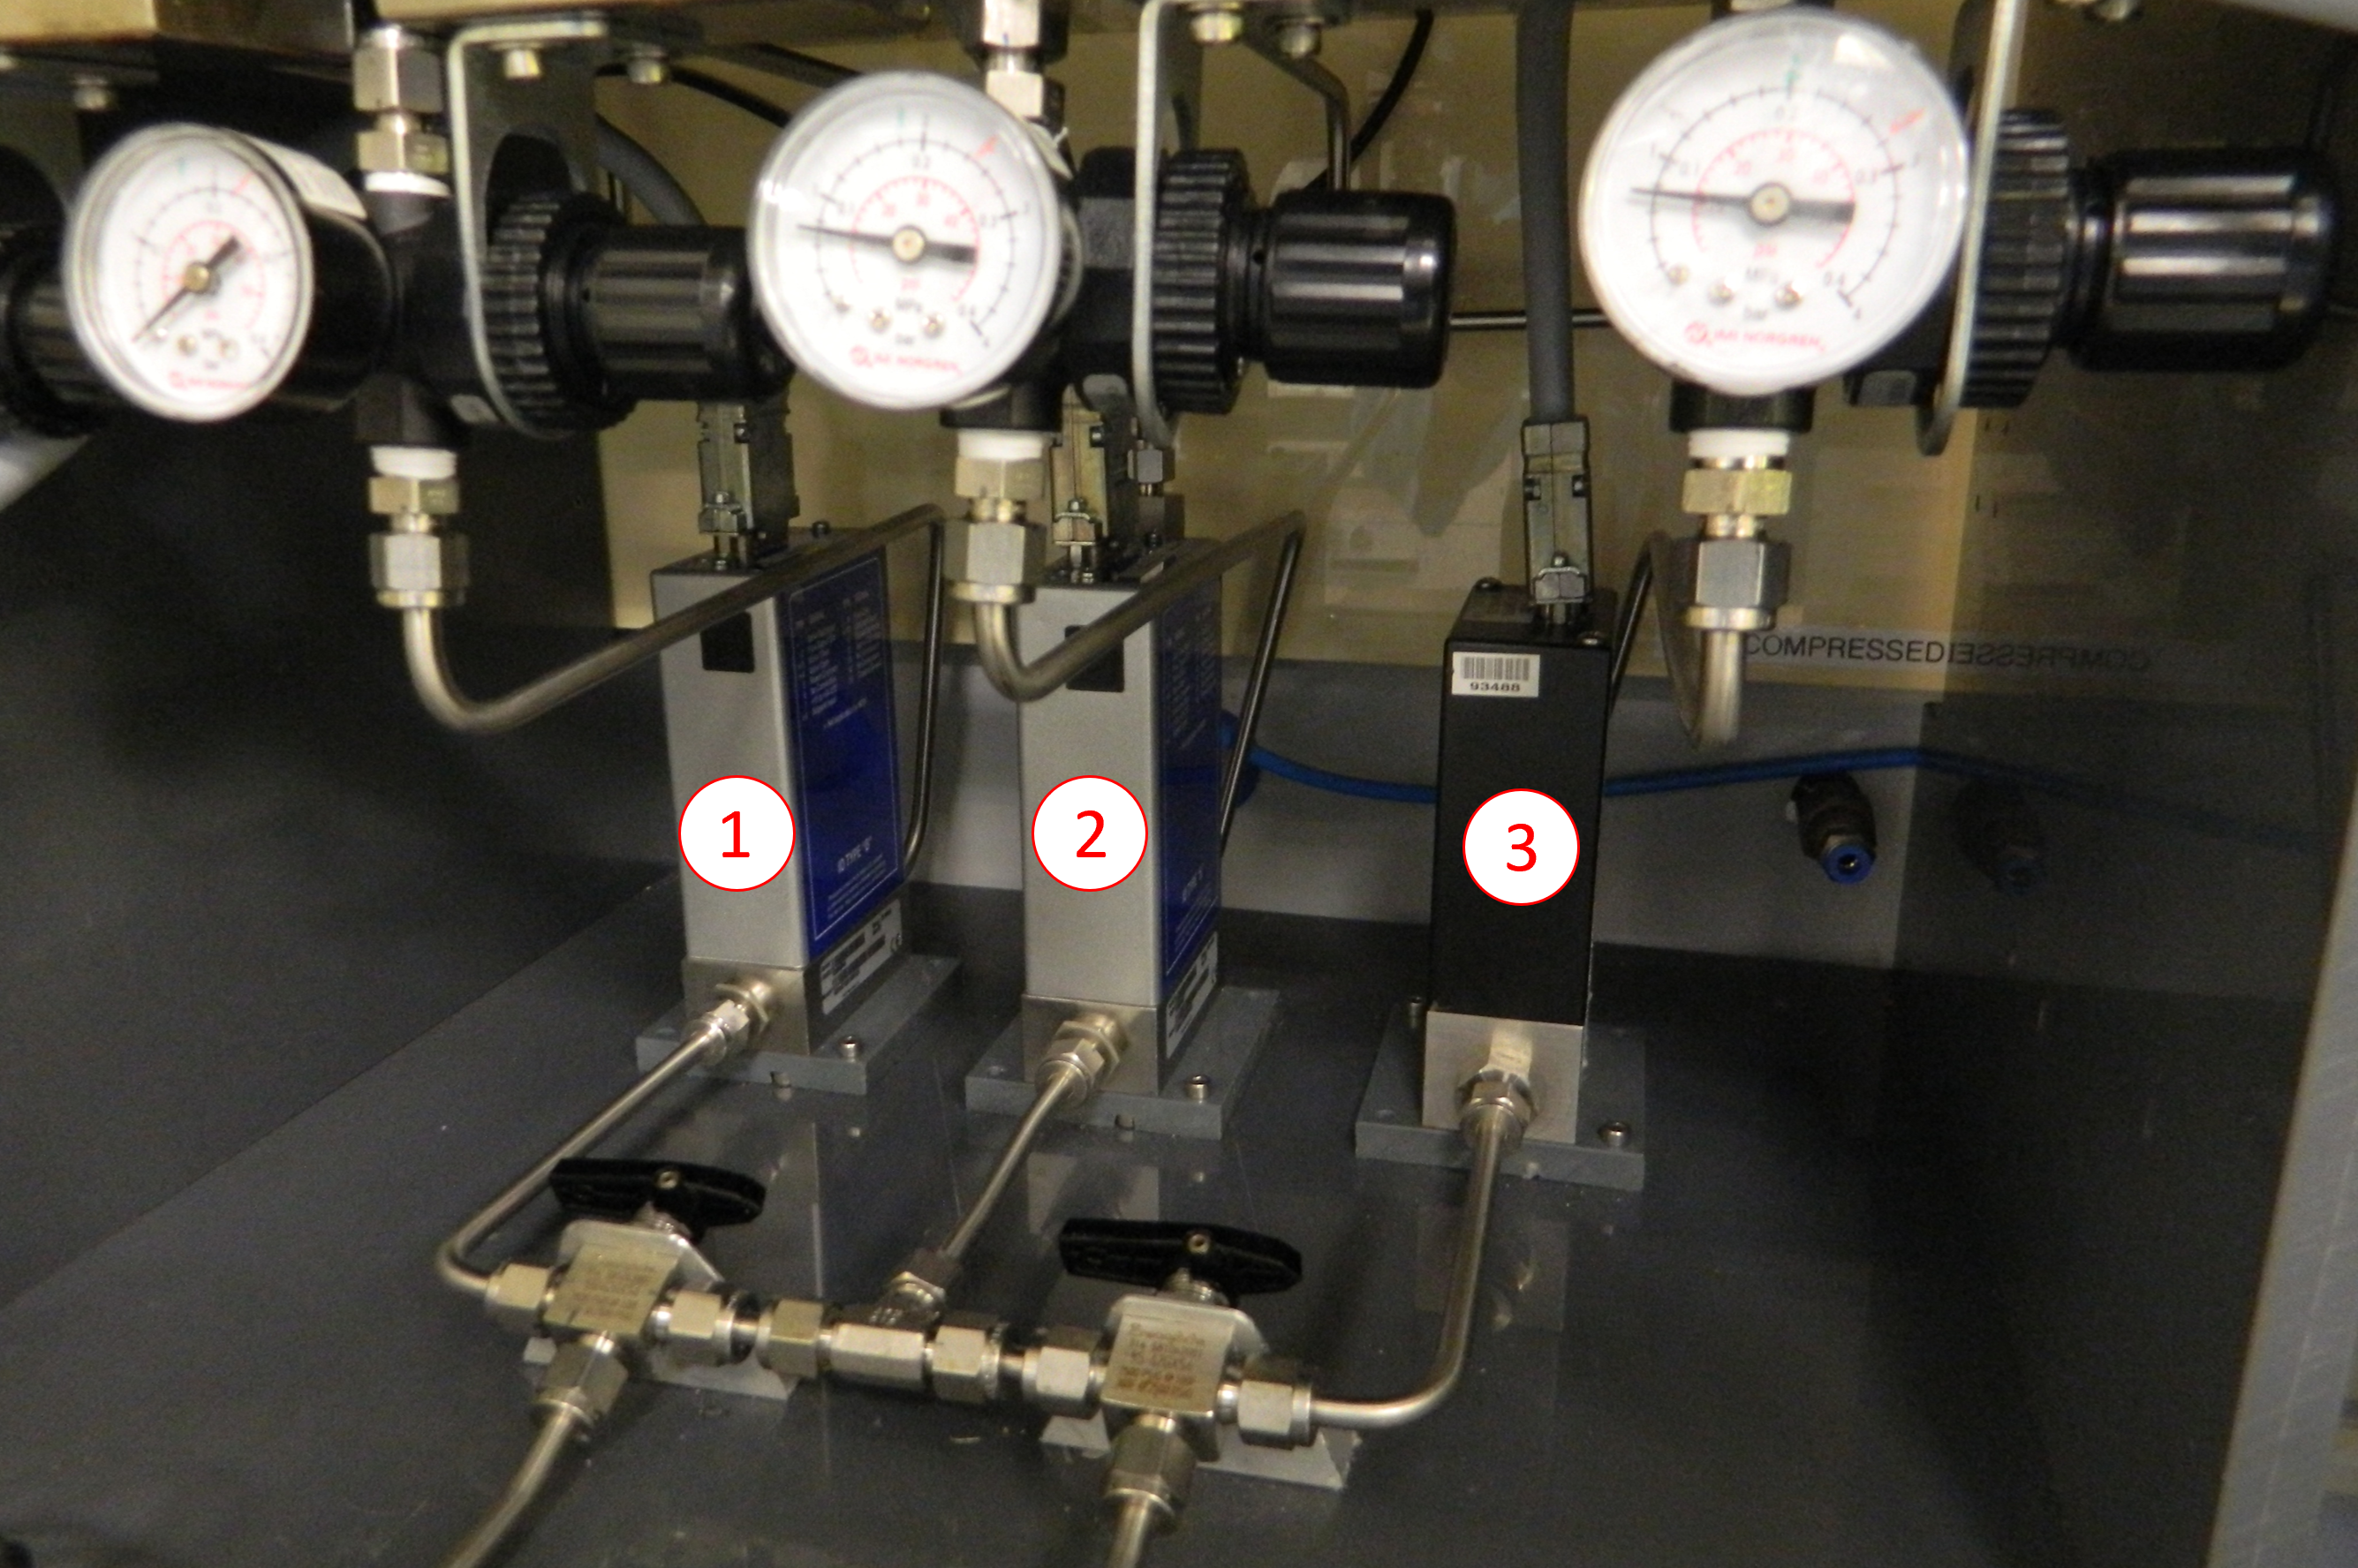
\includegraphics{figures/ch8/vapour_system_layout_2.png}

}

}

\end{minipage}%
%
\begin{minipage}[t]{0.15\linewidth}

{\centering 

~

}

\end{minipage}%
\newline
\begin{minipage}[t]{0.11\linewidth}

{\centering 

~

}

\end{minipage}%
%
\begin{minipage}[t]{0.03\linewidth}

{\centering 

\raisebox{-\height}{

\includegraphics{figures/(b).png}

}

}

\end{minipage}%
%
\begin{minipage}[t]{0.01\linewidth}

{\centering 

~

}

\end{minipage}%
%
\begin{minipage}[t]{0.70\linewidth}

{\centering 

\raisebox{-\height}{

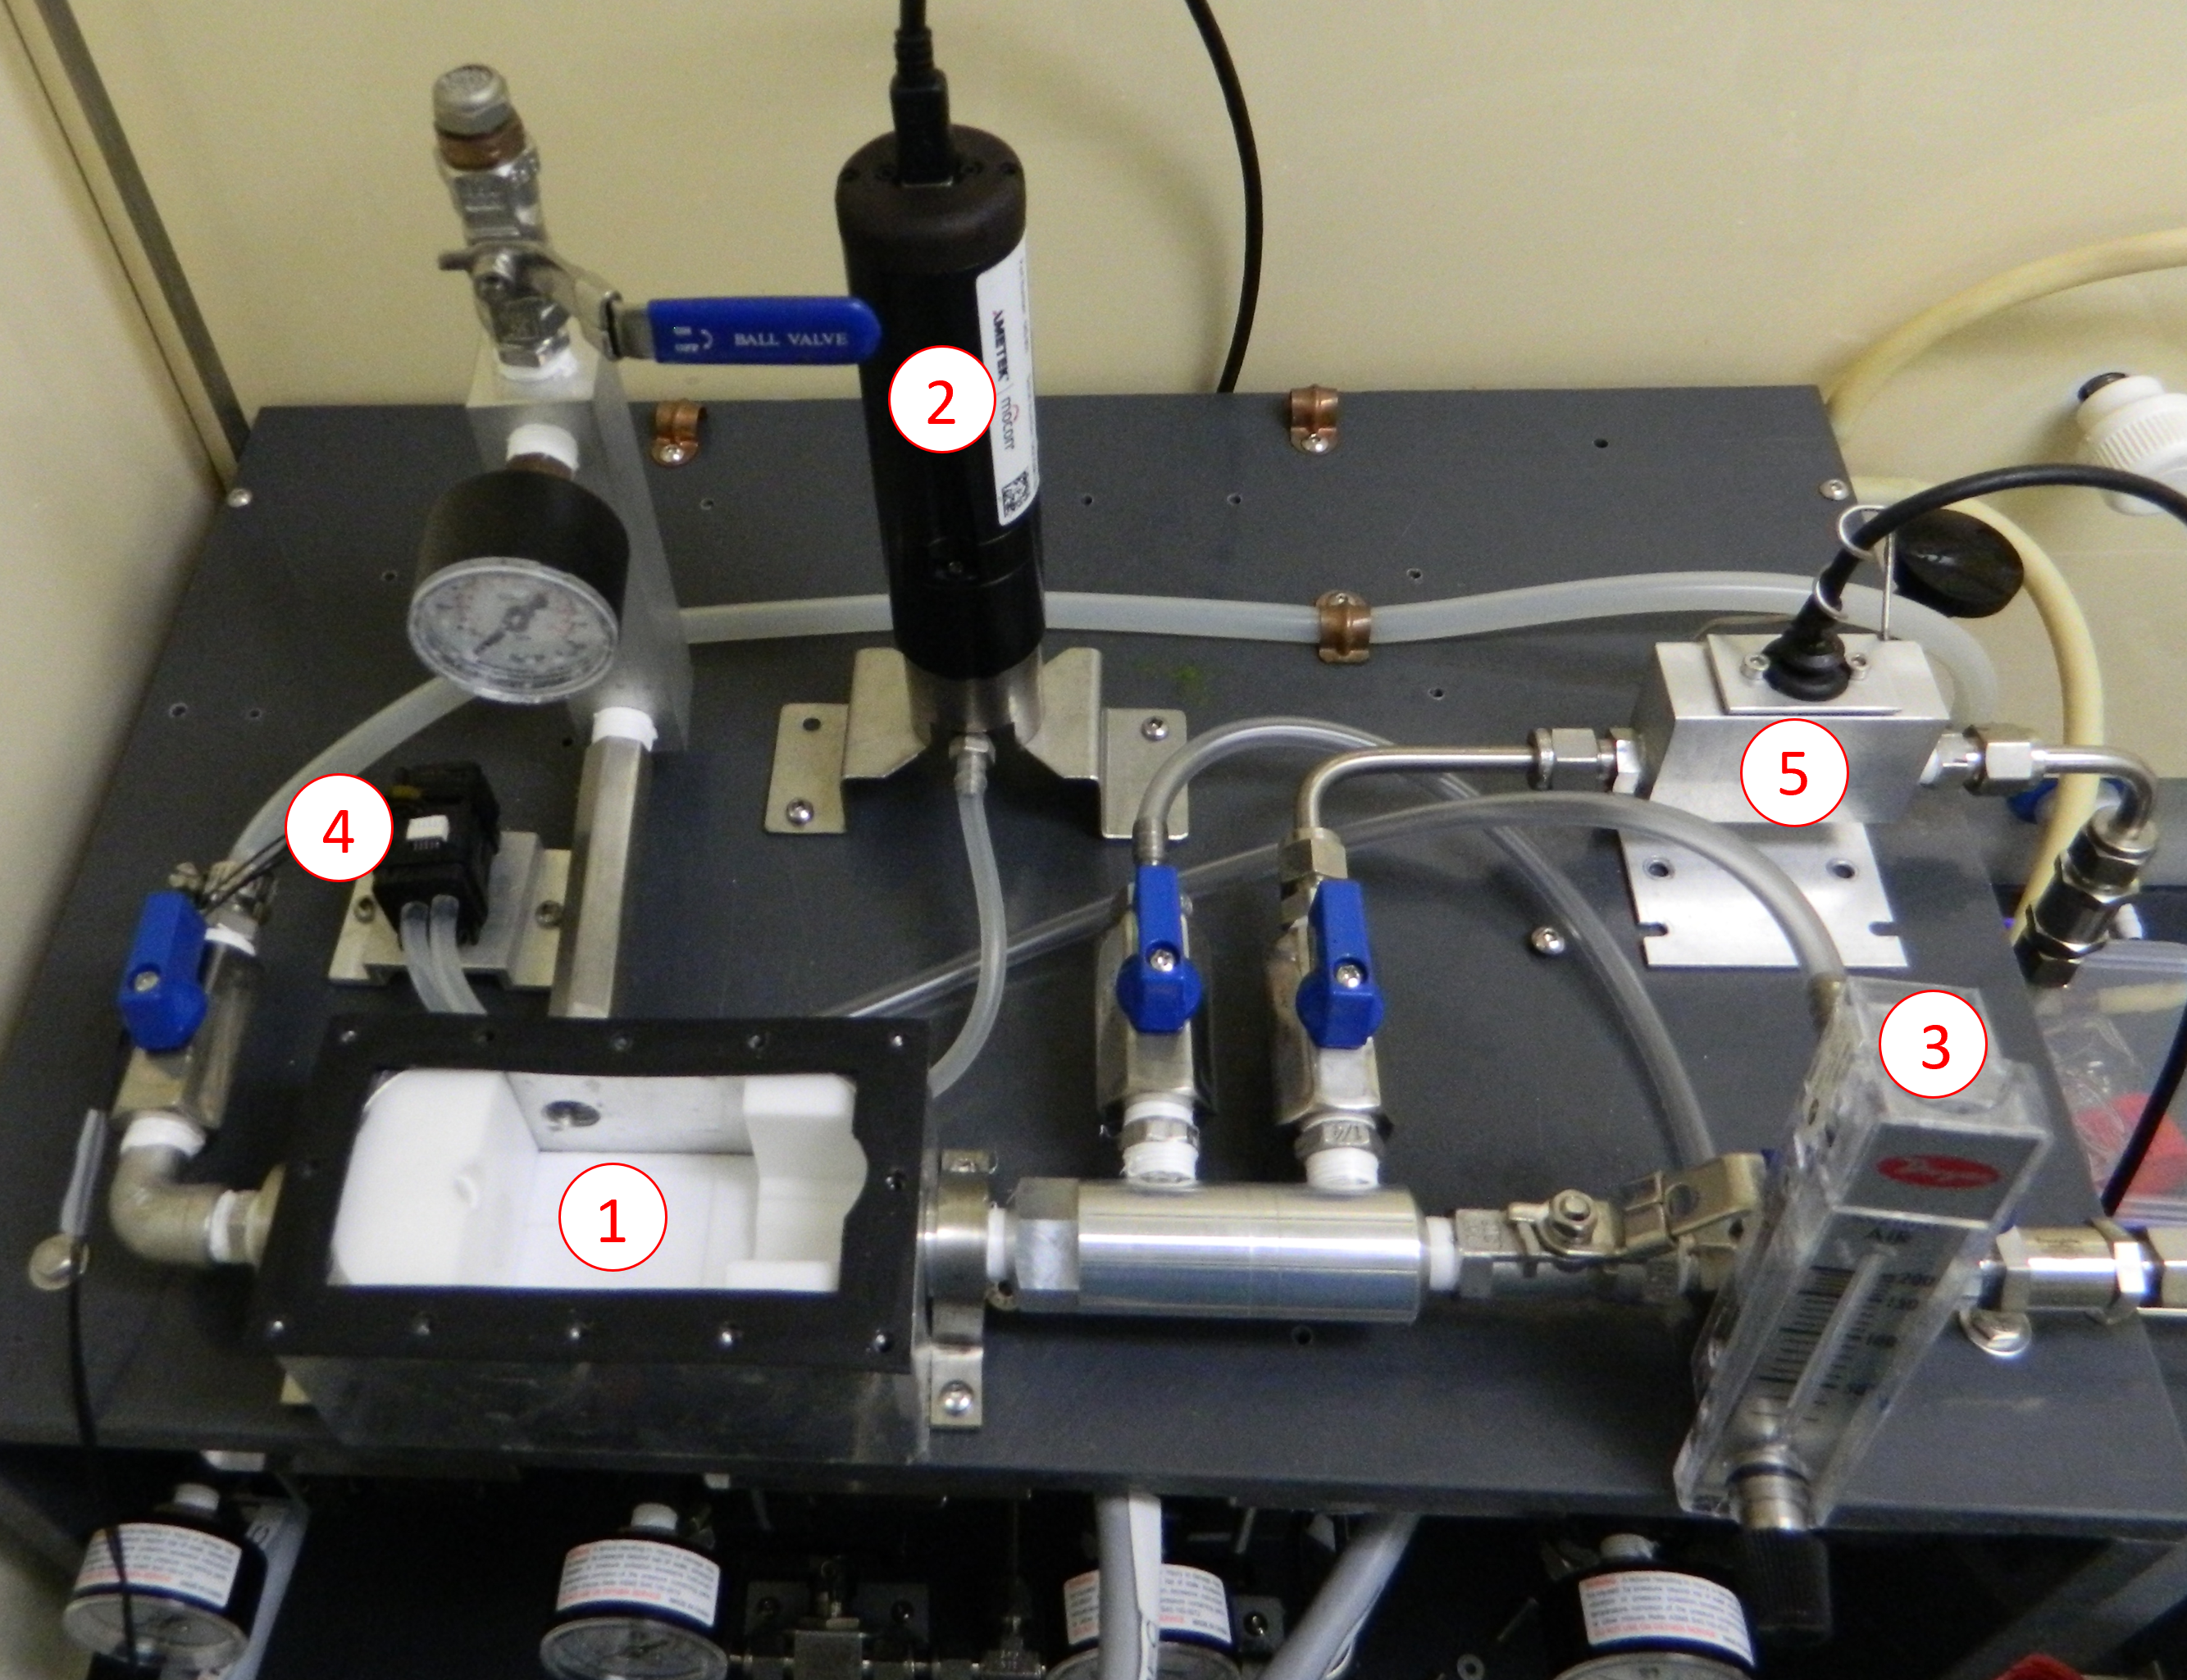
\includegraphics{figures/ch8/vapour_system_layout_1.png}

}

}

\end{minipage}%
%
\begin{minipage}[t]{0.15\linewidth}

{\centering 

~

}

\end{minipage}%

\caption{\label{fig-delivery-system}The three mass flow controllers
(MFCs) of the vapour delivery system are shown in (a), each with a
regulator to set the pressure at the MFC inlet. (1) is the 20 sccm
full-scale flow MFC, (2) is the 200 sccm full-scale flow MFC, and (3) is
the 500 sccm full-scale flow MFC. The device chamber, reference sensors
and other chamber peripherals are shown in (b). The components are
labelled as follows: (1) Device chamber, (2) Photoionisation detector
(PID), (3) Flowmeter from chamber to PID, (4) Micropump from chamber to
PID, (5) Relative humidity and temperature monitor.}

\end{figure}

Three mass flow controllers (MFCs) and their associated regulators sit
in a covered enclosure, seen from the front in
Figure~\ref{fig-delivery-system} (a). The MFCs are used to control the
nitrogen flow rate through two delivery lines, the carrier line and
dilution line. Each line consists of a mix of stainless steel and
flexible PVC tubing, with various Swagelok fittings and valves; these
valves include check valves, to ensure there is no vapour backflow. The
system is designed so that only one MFC delivers flow through each line.
Furthermore, the mass flow controller with a full-scale flow of 500 sccm
(standard cubic centimeters per minute) can only be directed through the
dilution line, and the mass flow controller with a full-scale flow of 20
sccm can only be directed through the carrier line. The dilution and
carrier lines merge at a mixing point about a metre before the device
chamber, which contains the device being tested. Flow through the
carrier line is bubbled through a volatile compound within a sealed 10
mL Schott bottle (Duran). A three-way valve determines whether the
analyte vapour is then carried towards the mixing point or sent to the
system exhaust.

\hypertarget{sec-reference-sensors}{%
\subsection{Reference Sensors}\label{sec-reference-sensors}}

Two reference sensors were added to the vapour delivery setup to compare
the response to vapour by the fabricated sensor device with some
reference signal. These reference sensors are a Ametek Mocon
photoionisation detector and a Telaire relative humidity and temperature
indicator. The layout of these reference sensors (and their associated
peripherals) relative to the device chamber is shown in
Figure~\ref{fig-delivery-system} (b). These components are on a raised
platform directly above the mass flow controller enclosure. Vapour
flowing through the device chamber passes into a cylindrical manifold
with three outlets. One outlet is the system exhaust, one flows into
relative humidity indicator chamber, and one flows into the
photoionisation detector. A dial-controlled micro diaphragm pump is used
to set the flow rate from the manifold into the photoionisation
detector, with a flowmeter used to monitor this flow rate. The
electronic integration and programming of the relative humidity and
temperature indicator is described in Section~\ref{sec-control-system}.
The photoionisation detector was connected to a laptop directly via USB,
then controlled and monitored using the supplier-provided VOC-TRAQ II
software package.

\hypertarget{relative-humidity-and-temperature-indicator}{%
\subsubsection*{Relative Humidity and Temperature
Indicator}\label{relative-humidity-and-temperature-indicator}}
\addcontentsline{toc}{subsubsection}{Relative Humidity and Temperature
Indicator}

The relative humidity and temperature indicator used here is a
capacitive humidity sensor \autocite{Telairesensor}. It consists of a
capacitor with a hygroscopic polymer as the capacitor dielectric. As
room temperature water has a much larger dielectric constant than the
polymer dielectric, absorption of water by the polymer leads to
increased sensor capacitance \autocite{capacitivesensor}. The sensor
capacitance, corresponding to the amount of moisture absorbed by the
polymer and therefore the relative humidity, is then translated by the
sensor into a calibrated electronic output. This output is then
processed using the hardware and software described in
Section~\ref{sec-control-system} to give a value for the relative
humidity. The sensor has a quoted relative humidity (RH) accuracy of
\(\pm 2.0\)\% when RH is below 80\%, and has a quoted temperature
accuracy of 0.5 °C \autocite{Telairesensor}. The absolute humidity (AH),
the mass of water vapour within a set volume, can be calculated in
gm\(^{-3}\) using Equation~\ref{eq-absolute-humidity}.

\begin{equation}\protect\hypertarget{eq-absolute-humidity}{}{ 
AH = C\frac{P_W}{T}
}\label{eq-absolute-humidity}\end{equation}

Here, \(C = 2.16679\) gKJ\(^{-1}\), \(P_W\) is the water vapour pressure
(in Pa) and T is the temperature (in K) \autocite{humidityformula}. For
temperatures between -20 °C and 50 °C, water vapour pressure \(P_W\) (in
hPa) can be approximated using Equation~\ref{eq-water-vapour-pressure}.

\begin{equation}\protect\hypertarget{eq-water-vapour-pressure}{}{
P_W = RH \times A \times 10^{(mT/(T+T_{n}))}
}\label{eq-water-vapour-pressure}\end{equation}

ΩHere, RH is relative humidity, T is temperature in °C, \(A = 6.116441\)
hPa, \(m = 7.591386\) and \(T_{n}\) = 240.7263 °C
\autocite{humidityformula}.

\hypertarget{photoionisation-detector}{%
\subsubsection*{Photoionisation
Detector}\label{photoionisation-detector}}
\addcontentsline{toc}{subsubsection}{Photoionisation Detector}

A photoionisation detector (PID) can be used to continuously monitor
volatile organic compounds by measuring the extent to which vapour
molecules passing through the detector can be ionised by incident UV
radiation. A small percentage of vapour molecules flowing into the
detector diffuse into a sensor cavity. This cavity is bounded on each
side by a pair of electrodes. A lamp in the body of the detector
radiates UV light through a window into this cavity. The vapour
molecules have their outer-most electrons excited and removed when
struck with these high-energy photons. The ionised molecules then drift
towards the sensor cathode, while free electrons drift towards the
sensor anode. This results in a current proportional to the
concentration of vapour molecules in the chamber. The current can then
be amplified for a signal readout. To be detected, the ionisation energy
of the molecules being monitored cannot exceed the energy of the
incident UV light. Therefore, molecules of clean air will not be
detected. Likewise, volatile organic compounds with high ionisation
energy \(-\) such as methane \(-\) will not be recognised by the PID.
Conversely, if the energy required to ionise a volatile of interest is
relatively low, the PID will generally show a relatively large response
to that volatile \autocite{Ionscience,PIDmanual}.

The Ametek Mocon photoionisation detector lamps used in this work each
had a lamp energy of 10.6 eV, with a quoted response time of less than 2
seconds. Photoionisation detectors are designed to sensitively detect
within a particular concentration range. PID sensors can become less
sensitive after being exposed to very high concentrations of volatile
gas. They can also become less sensitive if exposed to high levels of
humidity or volatile substances known to contaminate the PID window,
which are not used in this thesis. The typical sensitivity range of a
PID can be stated in terms of the sensor response to isobutylene gas,
which is typically used to calibrate PID sensors. The sensitivity ranges
of the two PID sensors used here were 10 ppb \(-\) 200 ppm and 100 ppb
\(-\) 2,000 ppm. Calibration with a reference gas ensures the detector
reads the true concentration of volatiles being detected, multiplied by
some previously-documented factor called a `response factor'. However,
these response factors can vary based on the design of the PID and
various environmental factors \autocite{Ionscience,PIDmanual}.

In this work, the PID was operated without end-user calibration. PID
measurements were used to confirm the evolution of vapour presence in
the chamber over time. It should be expected that sensor sensitivity
will exhibit span drift over days or weeks, depending on changes in the
local environment, and therefore measurements should not be treated as
absolute measurements that correspond to a true concentration reading. A
sampling rate of 1 s was used for all measurements. When sampling vapour
concentration, baseline measurements of nitrogen flow through the PID
were used as the zero concentration reference point. The vapour of
interest can be delivered to the PID either through diffusion or by
means of a low-power pump. A micro diaphragm pump (Xavitech) was
selected to pump the vapour from the chamber into the PID detector. This
pump was selected for its relatively low maximum flow rate, since the
PID requires an inlet flow of less than 300 sccm. As the pump is
controlled using an unlabelled dial, a flowmeter was used to
independently measure the flow rate through the micropump into the PID.

\hypertarget{sec-control-system}{%
\subsection{Control System}\label{sec-control-system}}

The vapour delivery system was controlled and monitored from a laptop
connected to a National Instruments USB-6009 multifunction data
acquisition input/output module (DAQ). This USB-6009 DAQ connected to
the mass flow controllers and relative humidity and temperature
indicator via a custom-designed circuit board manufactured by PCBway.
The outputs and inputs of the USB-6009 DAQ were set using custom LabView
software. These electronic and software components of the vapour
delivery control system are described in more detail below. The
photoionisation detector was controlled from the same laptop with its
own prepackaged software (VOC-TRAQ II).

\hypertarget{electronics}{%
\subsubsection*{Electronics}\label{electronics}}
\addcontentsline{toc}{subsubsection}{Electronics}

\begin{figure}

\begin{minipage}[t]{0.03\linewidth}

{\centering 

\raisebox{-\height}{

\includegraphics{figures/(a).png}

}

}

\end{minipage}%
%
\begin{minipage}[t]{0.01\linewidth}

{\centering 

~

}

\end{minipage}%
%
\begin{minipage}[t]{0.45\linewidth}

{\centering 

\raisebox{-\height}{

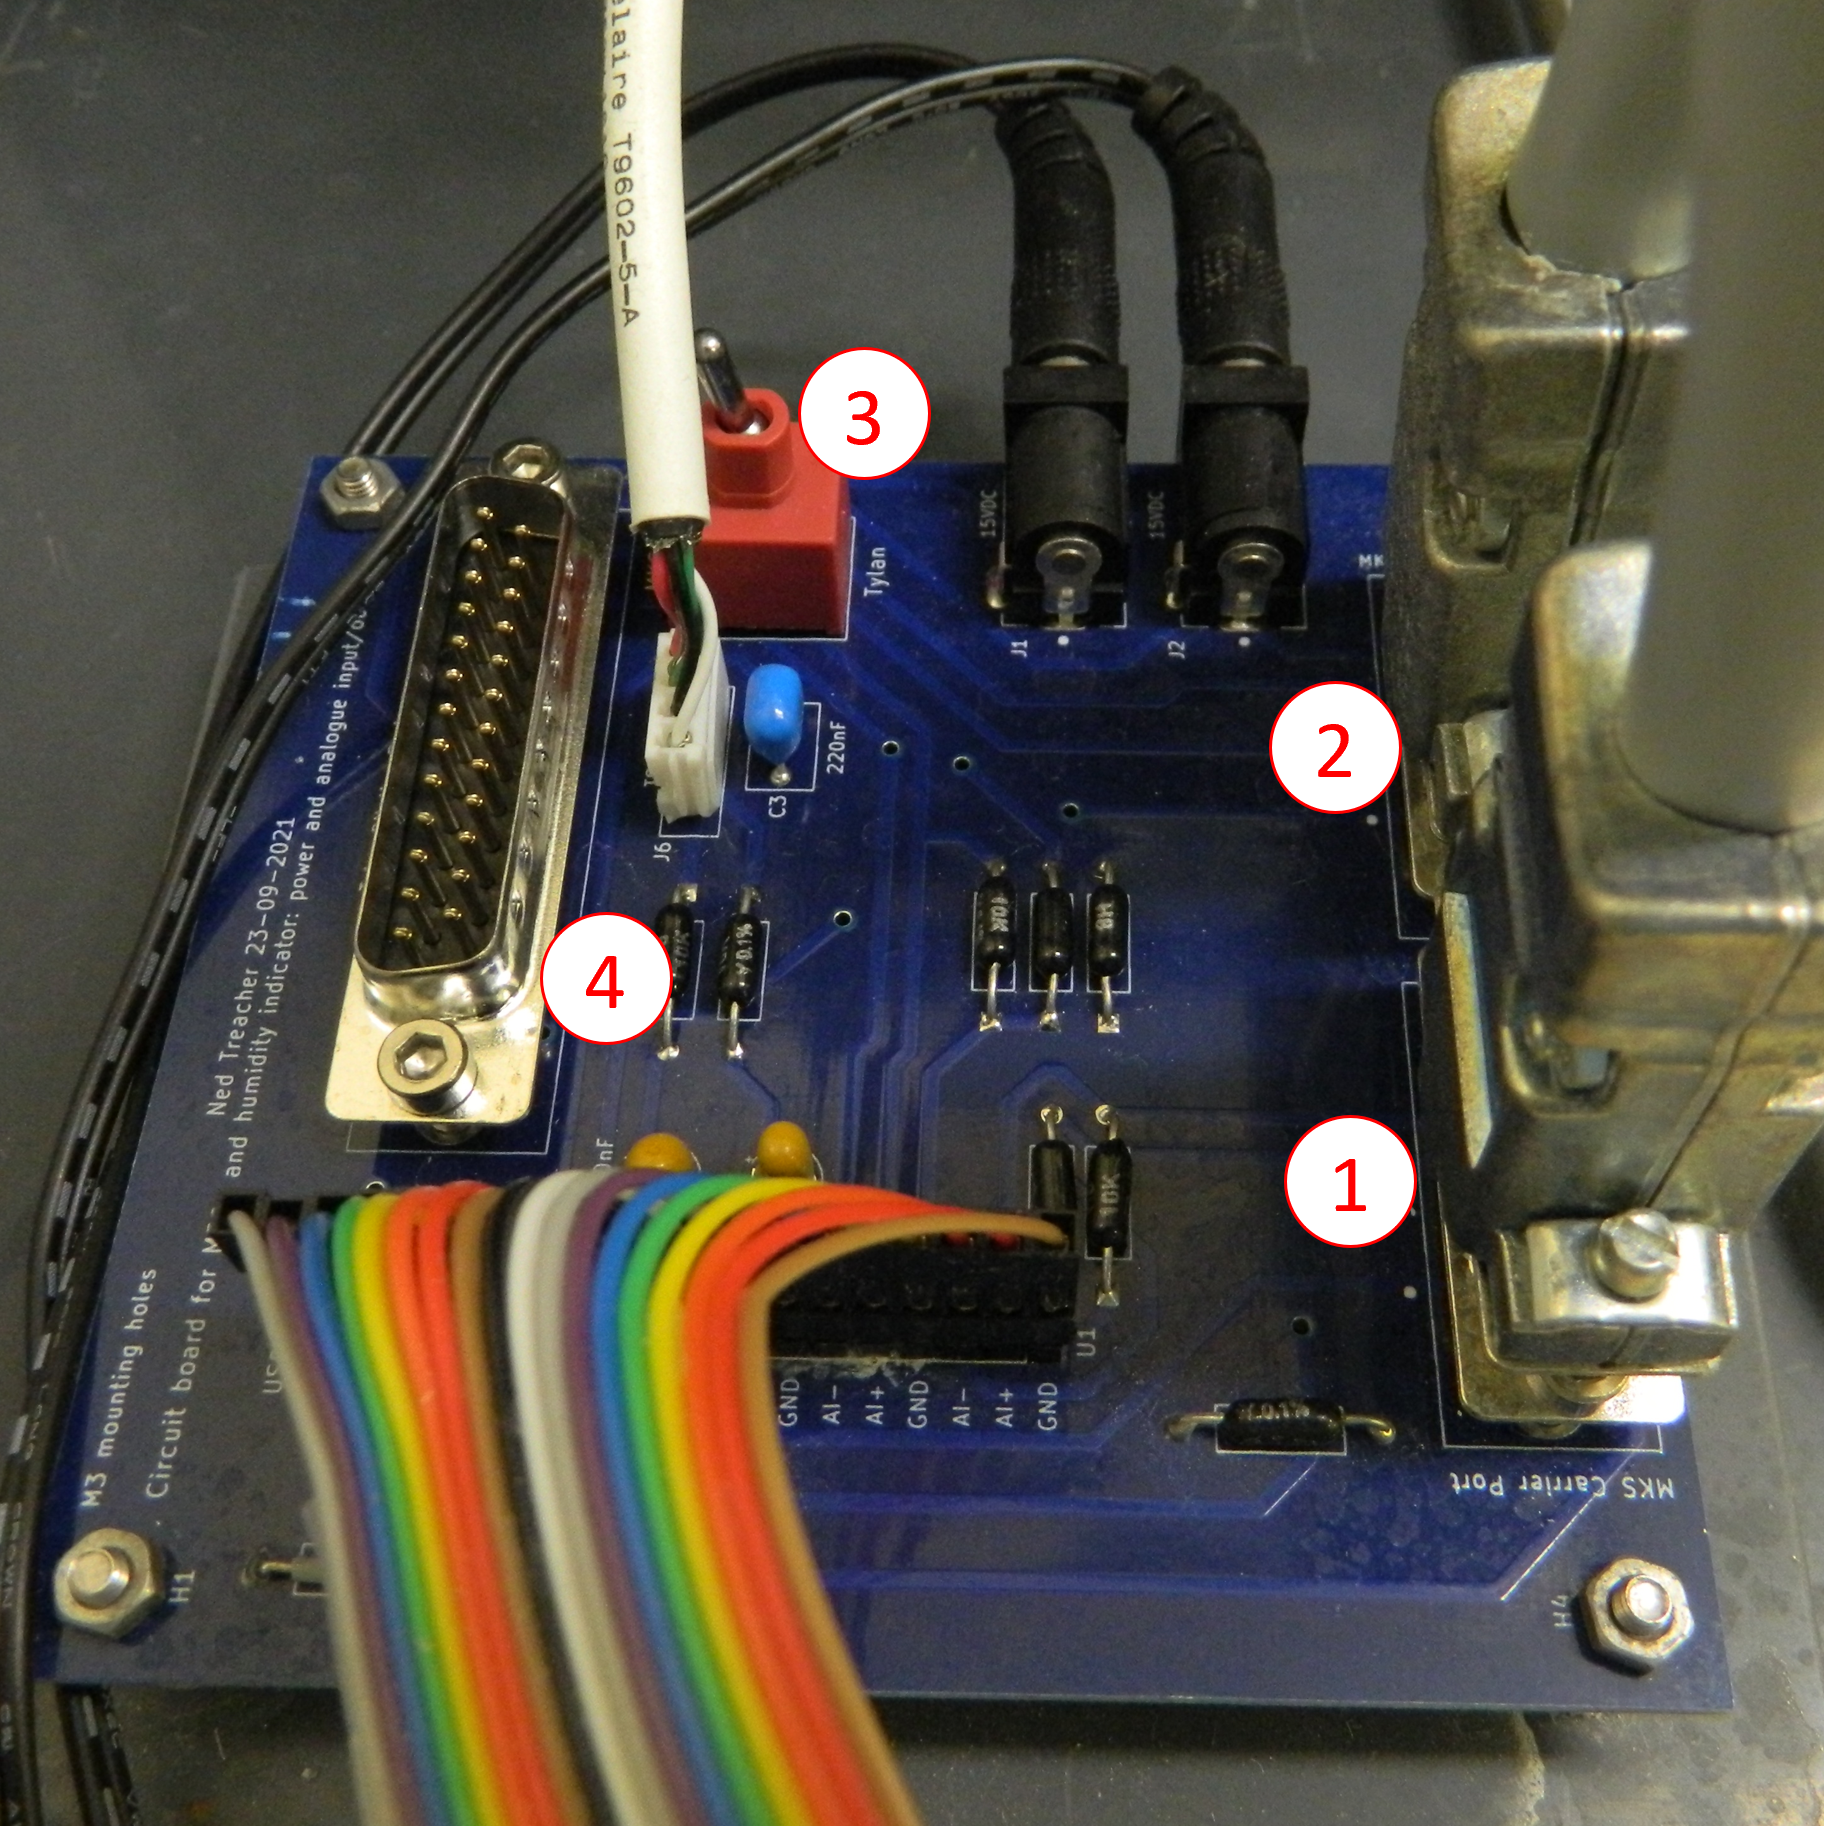
\includegraphics{figures/ch8/low_flow_config.png}

}

}

\end{minipage}%
%
\begin{minipage}[t]{0.01\linewidth}

{\centering 

~

}

\end{minipage}%
%
\begin{minipage}[t]{0.03\linewidth}

{\centering 

\raisebox{-\height}{

\includegraphics{figures/(b).png}

}

}

\end{minipage}%
%
\begin{minipage}[t]{0.01\linewidth}

{\centering 

~

}

\end{minipage}%
%
\begin{minipage}[t]{0.45\linewidth}

{\centering 

\raisebox{-\height}{

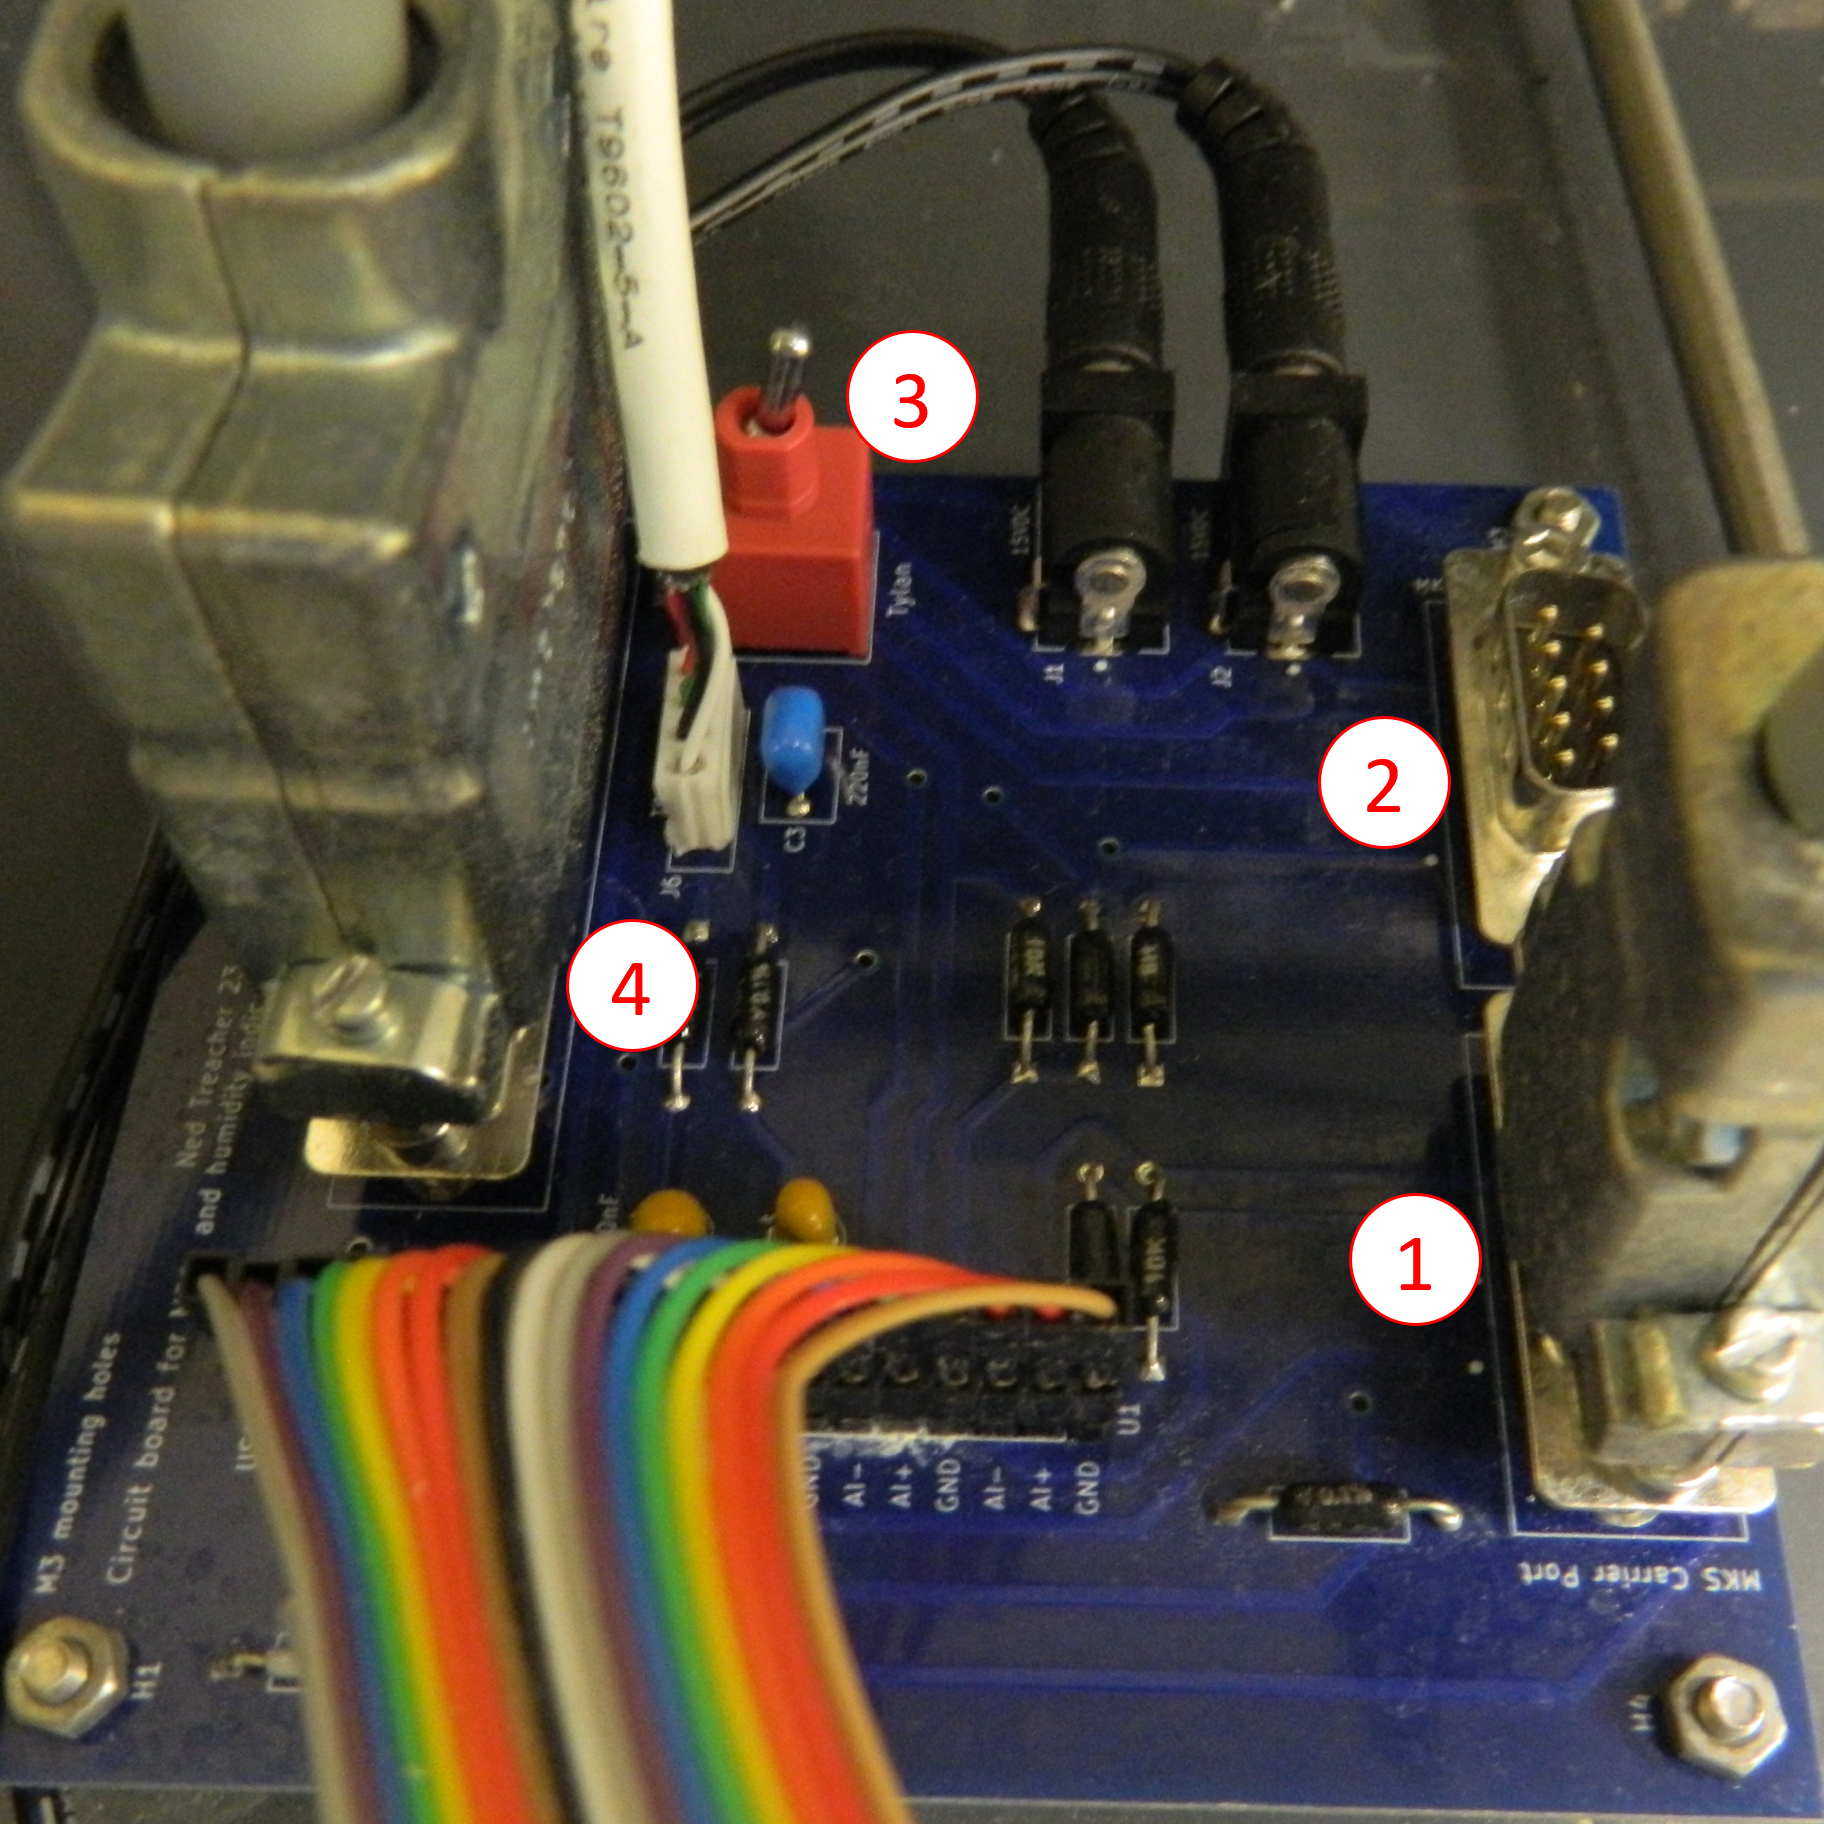
\includegraphics{figures/ch8/high_flow_config.png}

}

}

\end{minipage}%
%
\begin{minipage}[t]{0.01\linewidth}

{\centering 

~

}

\end{minipage}%

\caption{\label{fig-vapour-sensor-pcb}Images of the vapour delivery
control system circuit board, where (a) shows the low-flow configuration
and (b) shows the high-flow configuration. Components are labelled as
follows: (1) 9-pin carrier line port, (2) 9-pin dilution line port, (3)
red dilution port switch (determines which dilution line port is
active), (4) 25-pin dilution line port.}

\end{figure}

\begin{figure}

{\centering \includegraphics[width=0.95\textwidth,height=\textheight]{figures/ch8/current_PCB.png}

}

\caption{\label{fig-current-pcb-design}Circuit board schematic for
controlling and monitoring both the mass flow controllers and the
relative humidity and temperature sensor. Resistors R1-R6 are all 10
k\(\si{\ohm}\), while R7-R8 are both 0 \(\si{\ohm}\). The circuit board
was designed using the KiCad Layout Editor.}

\end{figure}

Figure~\ref{fig-vapour-sensor-pcb} shows the control circuit board
required to connect the mass flow controllers and relative humidity
indicator to the NI USB-6009. Only one mass flow controller can be set
to provide flow to a specific line. Therefore, only two mass flow
controllers can be operational simultaneously during testing. The
control circuit board allows the user to select the two mass flow
controllers to be used during a specific test run.
Figure~\ref{fig-vapour-sensor-pcb} (a) shows the `high-flow'
configuration, where the 500 sccm full-scale MFC is connected at the
25-pin dilution line port, the 200 sccm full-scale MFC is connected to
the 9-pin carrier line port, and red dilution port switch is towards
`Tylan' (rightwards). Figure~\ref{fig-vapour-sensor-pcb} (b) shows the
`low-flow' configuration, where the 200 sccm full-scale MFC is connected
to the 9-pin dilution line port, the 20 sccm full-scale MFC is connected
to the 9-pin carrier line port and the red dilution port switch is
towards `MKS' (leftwards). The design for the circuit board is shown in
Figure~\ref{fig-current-pcb-design}, showing the USB-6009 pinout. The
relative humidity and temperature sensor is connected to the circuit
board via the T9602 footprint. In the `high-flow' configuration, the
Tylan dilution and MKS carrier ports are connected to the corresponding
MFCs, with switch SW1 is towards `Tylan'. In the `low-flow'
configuration, both MKS ports are connected, and switch SW1 is towards
`MKS'.

\hypertarget{software}{%
\subsubsection*{Software}\label{software}}
\addcontentsline{toc}{subsubsection}{Software}

Two LabView Virtual Instruments (VIs) were adapted from pre-existing VIs
for operating the mass flow controllers and monitoring vapour flow into
the device chamber, as well as monitoring temperature and humidity in
the vapour delivery system's manifold. These VIs were named
`vapour-sensor-basic.vi' and `temp-and-humidity-basic.vi'. A third VI
was developed in parallel which combined the first two Virtual
Instruments and allowed the user to set a sequence of values for the
output flow from the mass flow controllers before an experimental run.
This VI was named `vapour-sensor-sequence-timestamped.vi'. Flow rate,
relative humidity and temperature data were then saved as .lvm files.
The LabView VIs described here are available on request.

\hypertarget{sec-vapour-system-design}{%
\section{Design}\label{sec-vapour-system-design}}

\hypertarget{initial-design}{%
\subsection{Initial Design}\label{initial-design}}

\begin{figure}

{\centering \includegraphics[width=1\textwidth,height=\textheight]{figures/ch8/PID_V0.png}

}

\caption{\label{fig-original-pid}P\&ID of the original vapour delivery
system}

\end{figure}

The initial design of the vapour delivery system, as shown in
Figure~\ref{fig-original-pid}, was relatively simple. No reference
sensors were included in the setup, and only one channel could be
characterised without opening the chamber and changing the position of
the device. However, as constructed it worked well as a self-contained
system, which was able to deliver vapour to a device channel while
measuring current across the channel. A 500 sccm full-range MFC (Tylan)
was placed on the dilution line, and a 200 sccm full-range MFC (Tylan)
was placed on the carrier line. A glass container for analyte was
present on the carrier line, with a vapour trap upstream to collect any
backflow. The vapour trap was removed in later iterations due to the
presence of a check valve to prevent backflow. The device chamber and
mass flow controllers were connected to a laptop and an Agilent 4156C
semiconductor parameter analyser and controlled using LabView.

\hypertarget{sec-vapour-system-design-1}{%
\subsection{Stage I Design}\label{sec-vapour-system-design-1}}

\begin{figure}

{\centering \includegraphics[width=1\textwidth,height=\textheight]{figures/ch8/PID_V1.png}

}

\caption{\label{fig-stage-1-pid}P\&ID of the Stage I vapour delivery
system.}

\end{figure}

The first stage of the vapour delivery system redesign, as shown in
Figure~\ref{fig-stage-1-pid}, was implemented in Nov 2021. This system
introduced the ability to use a 20 sccm full-range MFC (MKS Instruments)
for carrier line flow and a 200 sccm full-range MFC (MKS Instruments)
for either carrier or dilution line flow, to give better control when
using low flow rates. The reference sensors were also implemented, with
each sensor connected in parallel to the chamber exhaust. Through
testing the system with ethanol and acetone as analytes, the following
issues with this implementation of the setup were identified:

\begin{itemize}
\item
  With the system connected to the lab supply of nitrogen, pressure
  changes in the line due to nitrogen use elsewhere in the lab impacted
  the pressure at the MFCs and the flow through the lines.
\item
  The pressure indicator used for the device chamber had a much wider
  range than the pressure reached before nitrogen began to leak out of
  the PVC tubing; this meant pressure changes in the chamber, resulting
  from closing the exit valves while nitrogen flow entered the chamber,
  did not register on the indicator.
\item
  The PID responded unexpectedly slowly to changes in vapour
  concentration in the chamber. For example, after acetone or ethanol
  vapour had been run through the chamber, running clean nitrogen
  through the system for 3 hours was required before the PID returned to
  a constant baseline reading.
\item
  There was no way to ensure the device chamber was free of analyte
  vapour before an experimental run aside from running nitrogen through
  the dilution line. After prolonged use, condensed analyte was
  sometimes visible in the PVC lines of the delivery system.
\end{itemize}

These issues, along with various minor structural and design issues,
were addressed in the second-stage implementation of the system.

\hypertarget{stage-ii-design}{%
\subsection{Stage II Design}\label{stage-ii-design}}

\begin{figure}

{\centering \includegraphics[width=1\textwidth,height=\textheight]{figures/ch8/PID_V2.png}

}

\caption{\label{fig-stage-2-pid}Process \& instrumentation diagram
(P\&ID) of the second-stage design for the vapour delivery system. Red
outlines indicate additions introduced to the system subsequent to the
first stage design.}

\end{figure}

Figure~\ref{fig-stage-2-pid} gives an overview of the second-stage
design for the vapour delivery system setup. This stage of the redesign
was implemented between Jan and May 2022. Changes from the first stage
included:

\begin{itemize}
\item
  The addition of a N\(_2\) cylinder (152D size) as the source of
  nitrogen for the system to replace the lab supply.
\item
  A pressure indicator with a lower pressure range was used, which could
  register pressure changes within the device chamber.
\item
  A chamber manifold was placed before the exhaust with outlets into the
  PID and RHI.
\item
  A micro diaphragm pump was introduced between the manifold and PID to
  supply the PID with vapour from the chamber, and a flowmeter was
  placed before the pump to measure the flow rate out of the chamber to
  the PID. The PID was then seen to respond quickly to system changes
  (discussed further in Section~\ref{sec-calibration}).
\item
  A piece of PVC tubing was placed at the PID outlet to limit air from
  the fumehood entering the PID when the micropump was off.
\item
  Valves were placed before all system components so that the device
  chamber and post-analyte bottle carrier line could be evacuated with a
  roughing pump without potentially affecting components.
\item
  Check valves were placed at the exhaust to prevent backflow from the
  roughing pump into the delivery system.
\end{itemize}

These changes largely addressed the issues identified in
Section~\ref{sec-vapour-system-design-1}.

\hypertarget{sec-calibration}{%
\section{Chamber Flow Calibration}\label{sec-calibration}}

\begin{figure}

{\centering \includegraphics[width=0.45\textwidth,height=\textheight]{figures/ch8/water_displacement.png}

}

\caption{\label{fig-water-displacement}Setup for calibration of mass
flow controllers using the water displacement method.}

\end{figure}

A water displacement test was carried out to determine the relationship
between the flow rate measured by the mass flow controllers and the
actual flow rate passing through the chamber. All valves were set so
that both the dilution and carrier lines followed a single path. Both
these paths went through the device chamber and out through the system
exhaust. An empty analyte bottle was placed on the carrier line. The
system exhaust was placed into a bucket filled with tap water, with the
outlet sitting beneath an upturned 500 mL measurement cylinder, as
pictured in Figure~\ref{fig-water-displacement}. The cylinder was used
to measure the volume of displaced water over time, which is equivalent
to the rate of change of nitrogen volume entering the cylinder from the
exhaust. Measurements were taken from the bottom of the meniscus of the
water in the cylinder. As leaks from the manifold, chamber and exhaust
line were not detected when leak testing with bubble solution, it can be
safely assumed that the rate at which nitrogen exits the exhaust is
equivalent to the nitrogen flow rate through the device chamber.

\begin{figure}

\begin{minipage}[t]{0.03\linewidth}

{\centering 

\raisebox{-\height}{

\includegraphics{figures/(a).png}

}

}

\end{minipage}%
%
\begin{minipage}[t]{0.01\linewidth}

{\centering 

~

}

\end{minipage}%
%
\begin{minipage}[t]{0.45\linewidth}

{\centering 

\raisebox{-\height}{

\includegraphics{figures/ch8/200sccmMFC_carrierline_thruchamber.png}

}

}

\end{minipage}%
%
\begin{minipage}[t]{0.01\linewidth}

{\centering 

~

}

\end{minipage}%
%
\begin{minipage}[t]{0.03\linewidth}

{\centering 

\raisebox{-\height}{

\includegraphics{figures/(b).png}

}

}

\end{minipage}%
%
\begin{minipage}[t]{0.01\linewidth}

{\centering 

~

}

\end{minipage}%
%
\begin{minipage}[t]{0.45\linewidth}

{\centering 

\raisebox{-\height}{

\includegraphics{figures/ch8/500sccmMFC_dilutionline_thruchamber.png}

}

}

\end{minipage}%
%
\begin{minipage}[t]{0.01\linewidth}

{\centering 

~

}

\end{minipage}%

\caption{\label{fig-MFC-calibration-curves}The nominal flow rate as
measured by the mass flow controller compared to the actual flow rate
measured using water displacement testing, shown for the 200 sccm
full-scale mas flow controller placed through the carrier line in (a),
and for the 500 sccm full-scale mass flow controller placed through the
dilution line in (b). Three water displacement tests were performed for
each constant flow rate.}

\end{figure}

The time taken to displace 50 mL of water was measured three times for a
series of constant flow rates, both for the 200 sccm MFC (MKS) on the
carrier line and the 500 sccm MFC (Tylan) on the dilution line. The
displacement flow rate corresponding to each measurement could then be
found by dividing volume by time. These measurements, of displacement
flow relative to nominal flow through the MFC, are shown in
Figure~\ref{fig-MFC-calibration-curves} (a) and (b) respectively. The
increased uncertainty for higher flow measurements is largely due to
rapid flows being more difficult to measure precisely. However,
increased instability of flow at higher flow rates may also contribute.
A strong linear relationship between the nominal flow reading and actual
flow was identified. A linear least-squares fit with 95\% confidence
interval was performed, where coefficients \(a_1\) and \(a_2\) were
found for the linear relationship \(D = a_1d + a_2\). Here, \(d\) is
nominal flow from the MFC and \(D\) is measured displacement flow. For
the 200 sccm MFC flow through the carrier line, values of
\(a_1 = 1.18\pm0.09\) and \(a_2 = -1\pm13\) were obtained, while for the
500 sccm MFC flow through the dilution line, values of
\(a_1 = 1.16\pm0.04\) and \(a_2 = -5\pm10\) were obtained.

It appears that the offset between the measured displacement flow and
nominal output flow is not due to leaks in the system, since the offset
indicates measured flow exceeds the nominal flow. Instead, the offset
appears to be a systematic error introduced by the electronics or
software used to record the output flow from the MFCs. The identical
offset between measured and nominal flow observed for each MFC, even
when placed on different lines to the chamber, further strengthens the
likelihood of the offset being due to the control side of the system.
Furthermore, as both the carrier and dilution MFCs show readings with
the same offset multiplier within a 95\% confidence interval, the same
offset should apply to a mixture of flows on each line. For example, a
200 sccm nominal flow through the dilution line from the 500 sccm
full-scale MFC should have a roughly identical actual flow rate to a 50
sccm nominal flow through the dilution line and a 150 sccm flow through
the carrier line.

\begin{figure}

{\centering \includegraphics[width=0.45\textwidth,height=\textheight]{figures/ch8/PID_flowmeter.png}

}

\caption{\label{fig-flowmeter-calibration}Comparison of flowmeter
readings with flow measurements from water displacement testing. Three
water displacement tests were performed for each constant flow rate.}

\end{figure}

The time taken to displace a fixed water volume was also measured three
times for a series of constant flow rates through the flowmeter from the
chamber to exhaust. A least-squares linear relationship was obtained
between flowmeter readings and actual displacement, as shown in
Figure~\ref{fig-flowmeter-calibration}. Expressing the relationship as
\(D = b_1f + b_2\), where \(f\) is the flowmeter reading and \(D\) is
measured displacement flow, values of \(b_1 = 0.85\pm0.2\) and
\(b_2 = -18\pm26\) were obtained. The flow as read from the flowmeter
became less stable for flows above 150 sccm and below 130 sccm,
increasing measurement uncertainty. To understand the cause of this
instability, flow through the chamber was placed directly through the
flowmeter without the micropump present. Relatively stable measurements
could then be achieved, indicating that the flow rate instability
results from the micropump used for vapour delivery. This flow
instability was particularly pronounced when the micropump was operated
outside the 130 \(-\) 150 sccm range. The micropump flow measured as 150
sccm on the flowmeter was generally used when measuring vapour flow
through the delivery system to the photoionisation detector.
Figure~\ref{fig-flowmeter-calibration} indicates 150 sccm on the
flowmeter corresponds to \(\sim\) 110 sccm of actual flow.

\hypertarget{conclusion}{%
\section{Conclusion}\label{conclusion}}

A custom vapour delivery system was made suitable for field-effect
biosensor work by ensuring a range of flows could be delivered through
the system and installing suitable reference sensors for comparing
signal measurements to the field-effect biosensors. Two new mass flow
controllers with different maximum flow rates and two reference sensors,
a relative humidity and temperature sensor and photoionisation detector,
were introduced to the system in a two-stage design process. A new
electronic control system and LabView software were designed and
constructed for the altered delivery system. The nitrogen flow through
the system was then calibrated using water displacement testing, and it
was verified that the reference sensors both worked as expected. The
improvements to the system were significant, meaning it was far more
versatile, reliable and robust. As the system is modular and accessible,
it is expected that improvements to the system will continue to be
implemented as the insect odorant receptor biosensing field matures.
Possible future iterations, inspired by similar vapour delivery systems
successfully used for odorant receptor biosensing work
\autocite{Terutsuki2020,Hirata2021}, are discussed in more detail in
\textbf{?@sec-future-work-vapour}.

The following chapter, \textbf{?@sec-vapour-biosensing-iORs}, tests the
behaviour of pristine and insect odorant receptor functionalised devices
when exposed to vapour within the device chamber of the vapour delivery
system. This behaviour is compared with the data collected from the
validated reference sensors during the device testing.

\cleardoublepage
\phantomsection
\addcontentsline{toc}{part}{Appendices}
\appendix

\hypertarget{vapour-system-hardware}{%
\chapter{Vapour System Hardware}\label{vapour-system-hardware}}

\hypertarget{tbl-vapour-sensor-components}{}
\begin{longtable}[]{@{}
  >{\raggedright\arraybackslash}p{(\columnwidth - 4\tabcolsep) * \real{0.5930}}
  >{\raggedright\arraybackslash}p{(\columnwidth - 4\tabcolsep) * \real{0.2209}}
  >{\raggedright\arraybackslash}p{(\columnwidth - 4\tabcolsep) * \real{0.1860}}@{}}
\caption{\label{tbl-vapour-sensor-components}Major components used in
construction of the vapour delivery system described in this
thesis.}\tabularnewline
\toprule\noalign{}
\begin{minipage}[b]{\linewidth}\raggedright
Description
\end{minipage} & \begin{minipage}[b]{\linewidth}\raggedright
Part No.
\end{minipage} & \begin{minipage}[b]{\linewidth}\raggedright
Manufacturer
\end{minipage} \\
\midrule\noalign{}
\endfirsthead
\toprule\noalign{}
\begin{minipage}[b]{\linewidth}\raggedright
Description
\end{minipage} & \begin{minipage}[b]{\linewidth}\raggedright
Part No.
\end{minipage} & \begin{minipage}[b]{\linewidth}\raggedright
Manufacturer
\end{minipage} \\
\midrule\noalign{}
\endhead
\bottomrule\noalign{}
\endlastfoot
Mass flow controller, 20 sccm full scale & GE50A-013201SBV020 & MKS
Instruments \\
Mass flow controller, 200 sccm full scale & GE50A-013202SBV020 & MKS
Instruments \\
Mass flow controller, 500 sccm full scale & FC-2901V & Tylan \\
Analogue flowmeter, 240 sccm max. flow & 116261-30 & Dwyer \\
Micro diaphragm pump & P200-B3C5V-35000 & Xavitech \\
Analogue flow controller, for micro diaphragm pump & X3000450 &
Xavitech \\
10 mL Schott bottle & 218010802 & Duran \\
PTFE connection cap system & Z742273 & Duran \\
Baseline VOC-TRAQ flow cell, purple & 043-950 & Ametek Mocon \\
Baseline VOC-TRAQ flow cell, red & 043-951 & Ametek Mocon \\
Humidity and temperature sensor & T9602-5-A & Telaire \\
\end{longtable}

\hypertarget{python-code-for-data-analysis}{%
\chapter{Python Code for Data
Analysis}\label{python-code-for-data-analysis}}

\hypertarget{code-repository}{%
\section{Code Repository}\label{code-repository}}

The code used for general analysis of field-effect transistor devices in
this thesis was written with Python 3.8.8. Contributors to the code used
include Erica Cassie, Erica Happe, Marissa Dierkes and Leo Browning. The
code is located on GitHub and the research group OneDrive, and is
available on request.

\hypertarget{sec-histogram-analysis}{%
\section{Atomic Force Microscope Histogram
Analysis}\label{sec-histogram-analysis}}

The purpose of this code is to analyse atomic force microscope (AFM)
images of carbon nanotube networks in .xyz format taken using an atomic
force microscope and processed in Gwyddion (see
\textbf{?@sec-afm-characterisation}). It was originally designed by
Erica Happe in Matlab, and adapted by Marissa Dierkes and myself for use
in Python. The code imports the .xyz data and sorts it into bins 0.15 nm
in size for processing. To perform skew-normal distribution fits, both
\emph{scipy.optimize.curve\_fit} and \emph{scipy.stats.skewnorm} modules
are used in this code.

\hypertarget{sec-raman-analysis}{%
\section{Raman Spectroscopy Analysis}\label{sec-raman-analysis}}

The purpose of this code is to analyse a series of Raman spectra taken
at different points on a single film (see
\textbf{?@sec-raman-characterisation}). Data is imported in a series of
tab-delimited text files, with the low wavenumber spectrum (100
cm\(^{-1} - 650\) cm\(^{-1}\)) and high wavenumber spectrum (1300
cm\(^{-1} - 1650\) cm\(^{-1}\)) imported in separate datafiles for each
scan location.

\hypertarget{sec-field-effect-transistor-analysis}{%
\section{Field-Effect Transistor
Analysis}\label{sec-field-effect-transistor-analysis}}

The purpose of this code is to analyse electrical measurements taken of
field-effect transistor (FET) devices. Electrical measurements were
either taken from the Keysight 4156C Semiconductor Parameter Analyser,
National Instruments NI-PXIe or Keysight B1500A Semiconductor Device
Analyser as discussed in \textbf{?@sec-electrical-characterisation}; the
code is able to analyse data in .csv format taken from all three
measurement setups. The main Python file in the code base consists of
three related but independent modules: the first analyses and plots
sensing data from the FET devices, the second analyses and plots
transfer characteristics from channels across a device, and the third
compares individual channel characteristics before and after a
modification or after each individual modification in a series of
modifications. The code base also features a separate config file and
style sheet which govern the behaviour of the main code. The code base
was designed collaboratively by myself and Erica Cassie over GitHub
using the Sourcetree Git GUI.

\hypertarget{references}{%
\chapter*{References}\label{references}}
\addcontentsline{toc}{chapter}{References}

\markboth{References}{References}

\printbibliography[heading=none]


\backmatter

\end{document}
